\chapter{Facility design}
    Since there was no existing LSP facility at McGill University, a considerable portion of this project revolved around the design and fabrication of an LSP generator. This is summarized in the following need statement:

    \begin{statement}{Need statement} 
        Experimental testing will be critical in the development of a laser-thermal propulsion (LTP) system. Thus, there is a need for a laboratory facility to study laser-sustained plasma and LTP thrust characteristics in conditions comparable to those expected in a working thruster.
    \end{statement}
    
    This chapter will discuss the major design requirements of such a system, the selection of appropriate solutions, and the assembly, integration, and testing process. Several practical issues were encountered in developing the LSP generator, which are rarely mentioned in the experimental LSP literature. They will be documented in detail in this report in the hopes that this can facilitate future work in this field.

    \section{Existing hardware and OTS components} \label{sec:design_ots}
        As seen in \autoref{sec:background_exp} and shown in \autoref{fig:exp_subsys}, an experimental LTP test facility consists of at least 5 subsystems:
        \begin{enumerate}
            \item A laser source and any beam-shaping optics
            \item A pressurized test section or thruster with a suitable ignition mechanism
            \item A feed system for the thruster/test section
            \item A thrust bench
            \item An instrumentation suite to measure pressure, flow rates, temperatures, thrust, etc.
        \end{enumerate}

        Most of the design activities revolved around subsystem number two: the test section. The laser, feed system, and instruments either were already available in the laboratory or purchased off-the-shelf (OTS). The thrust stand design was delegated to a team of students collaborating on this project.

        \begin{figure}[h]
            \centering
            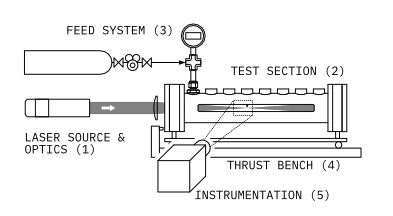
\includegraphics[]{assets/3 design/experiment_diagram}
            \caption[LTP Experiment subsystems]{LTP Experiment subsystems. The field of view of the high-speed camera is shown in dotted lines. Any snapshots from the camera shown in this report will be from this region.}
            \label{fig:exp_subsys}
        \end{figure}

        \subsection{Laser system}
            The laser made available for this project was the most important driver of many design decisions. Whether they are for interstellar-class lightsails as envisioned by \textcite{lubinRoadmapInterstellarFlight2016a}, or interplanetary missions powered by electric propulsion as proposed by \textcite{sheerinFastSolarSystem2021}, fiber lasers operating at the 1064-nm-wavelength are currently favored\added{, for both physical and economic reasons discussed in \autoref{sec:background_principle},} for many DEP applications. Since LTP is proposed as an additional DEP concept within this ecosystem, this experimental work aimed to match this laser wavelength.

            An IPG Photonics YLR-300/3000-QCW-MM-AC Ytterbium fiber laser (seen in \autoref{fig:laser_laser}) was generously loaned to the IFERG by the Royal Military College of Canada. This is an infrared laser primarily designed for welding, drilling, and cutting. It is capable of operating in both pulsed and continuous modes at a wavelength of \qty{1070}{nm}. Its key specifications are summarized in \autoref{tab:laser_spec}. A complete calibration report for the laser can be found in \autoref{chp:app_YLR}. An IPG Photonics P30-001736 collimator head (seen in \autoref{fig:laser_collimator}) was also acquired for the laser, forming a 1-in-diameter beam at its output. The collimator's calibration report can be found in \autoref{chp:app_Collimator}.

            \begin{table}[h]
                \centering
                \caption{Summary of nominal laser specifications}
                \label{tab:laser_spec}
                \begin{tabular}{@{}lrl@{}}
                    \toprule
                    Parameter            & Quantity & Unit \\ \midrule
                    Wavelength                    & 1070              & nm            \\
                    Maximum CW Power              & 300               & W             \\
                    Maximum Pulse Power           & 3000              & W             \\
                    Maximum Pulse Duration (3 kW) & 10                & ms            \\
                    Maximum Pulse Energy          & 30              & J             \\ \bottomrule
                    \end{tabular}
            \end{table}

            Although a practical LTP system would likely operate in continuous mode, the YLR laser's pulsed mode was of particular interest in this project. As discussed in \autoref{sec:background_lsp}, laser power is a critical factor in the ability to achieve a steady LSP. The YLR laser is not only capable of pulsing at an order of magnitude above its CW power rating, but it is able to do so for several milliseconds, a relatively long-pulse in the world of laser physics. This pulse is in fact so long that it is considered to be in the CW regime as far as laser damage is concerned (\textcite{thorlabsNBK7PlanoConvexLenses}), hence the \emph{Quasi}-Continuous-Wave (QCW) designation of this laser. This capability enables running very high-power experiments without investing in far more expensive (and dangerous) CW kW-class lasers, although the 10~ms timescale imposes a major constraint on the facility design and experimental methodology.

            \paragraph{Laser safety} \added{Considerations for safety were paramount in operating the high-power laser. All personnel involved in the project followed mandatory laser safety training prior to participating to experiments. A detailed laser operation procedure was posted at the laser control station and was included in the experiment procedure document (available in \autoref{chp:app_procedure}). Laser safety screens and safety curtains were used to minimize the risk of laser exposure. Laboratory personnel was instructed to wear appropriate laser-safety goggles. The experiment was designed to be operable without entering the laser curtain enclosure. Appropriate signage and light signals were placed outside the laboratory entrance to inform passersby of the presence and operation of a class-4 laser, as mandated by McGill-wide laser safety guidelines. A laser-safety officer was invited to visit the laboratory to vet the safety measures and provide recommendations that were promptly followed.}

            \begin{figure}[h]
                \centering
                \begin{subfigure}[t]{0.6\textwidth}
                    \centering
                    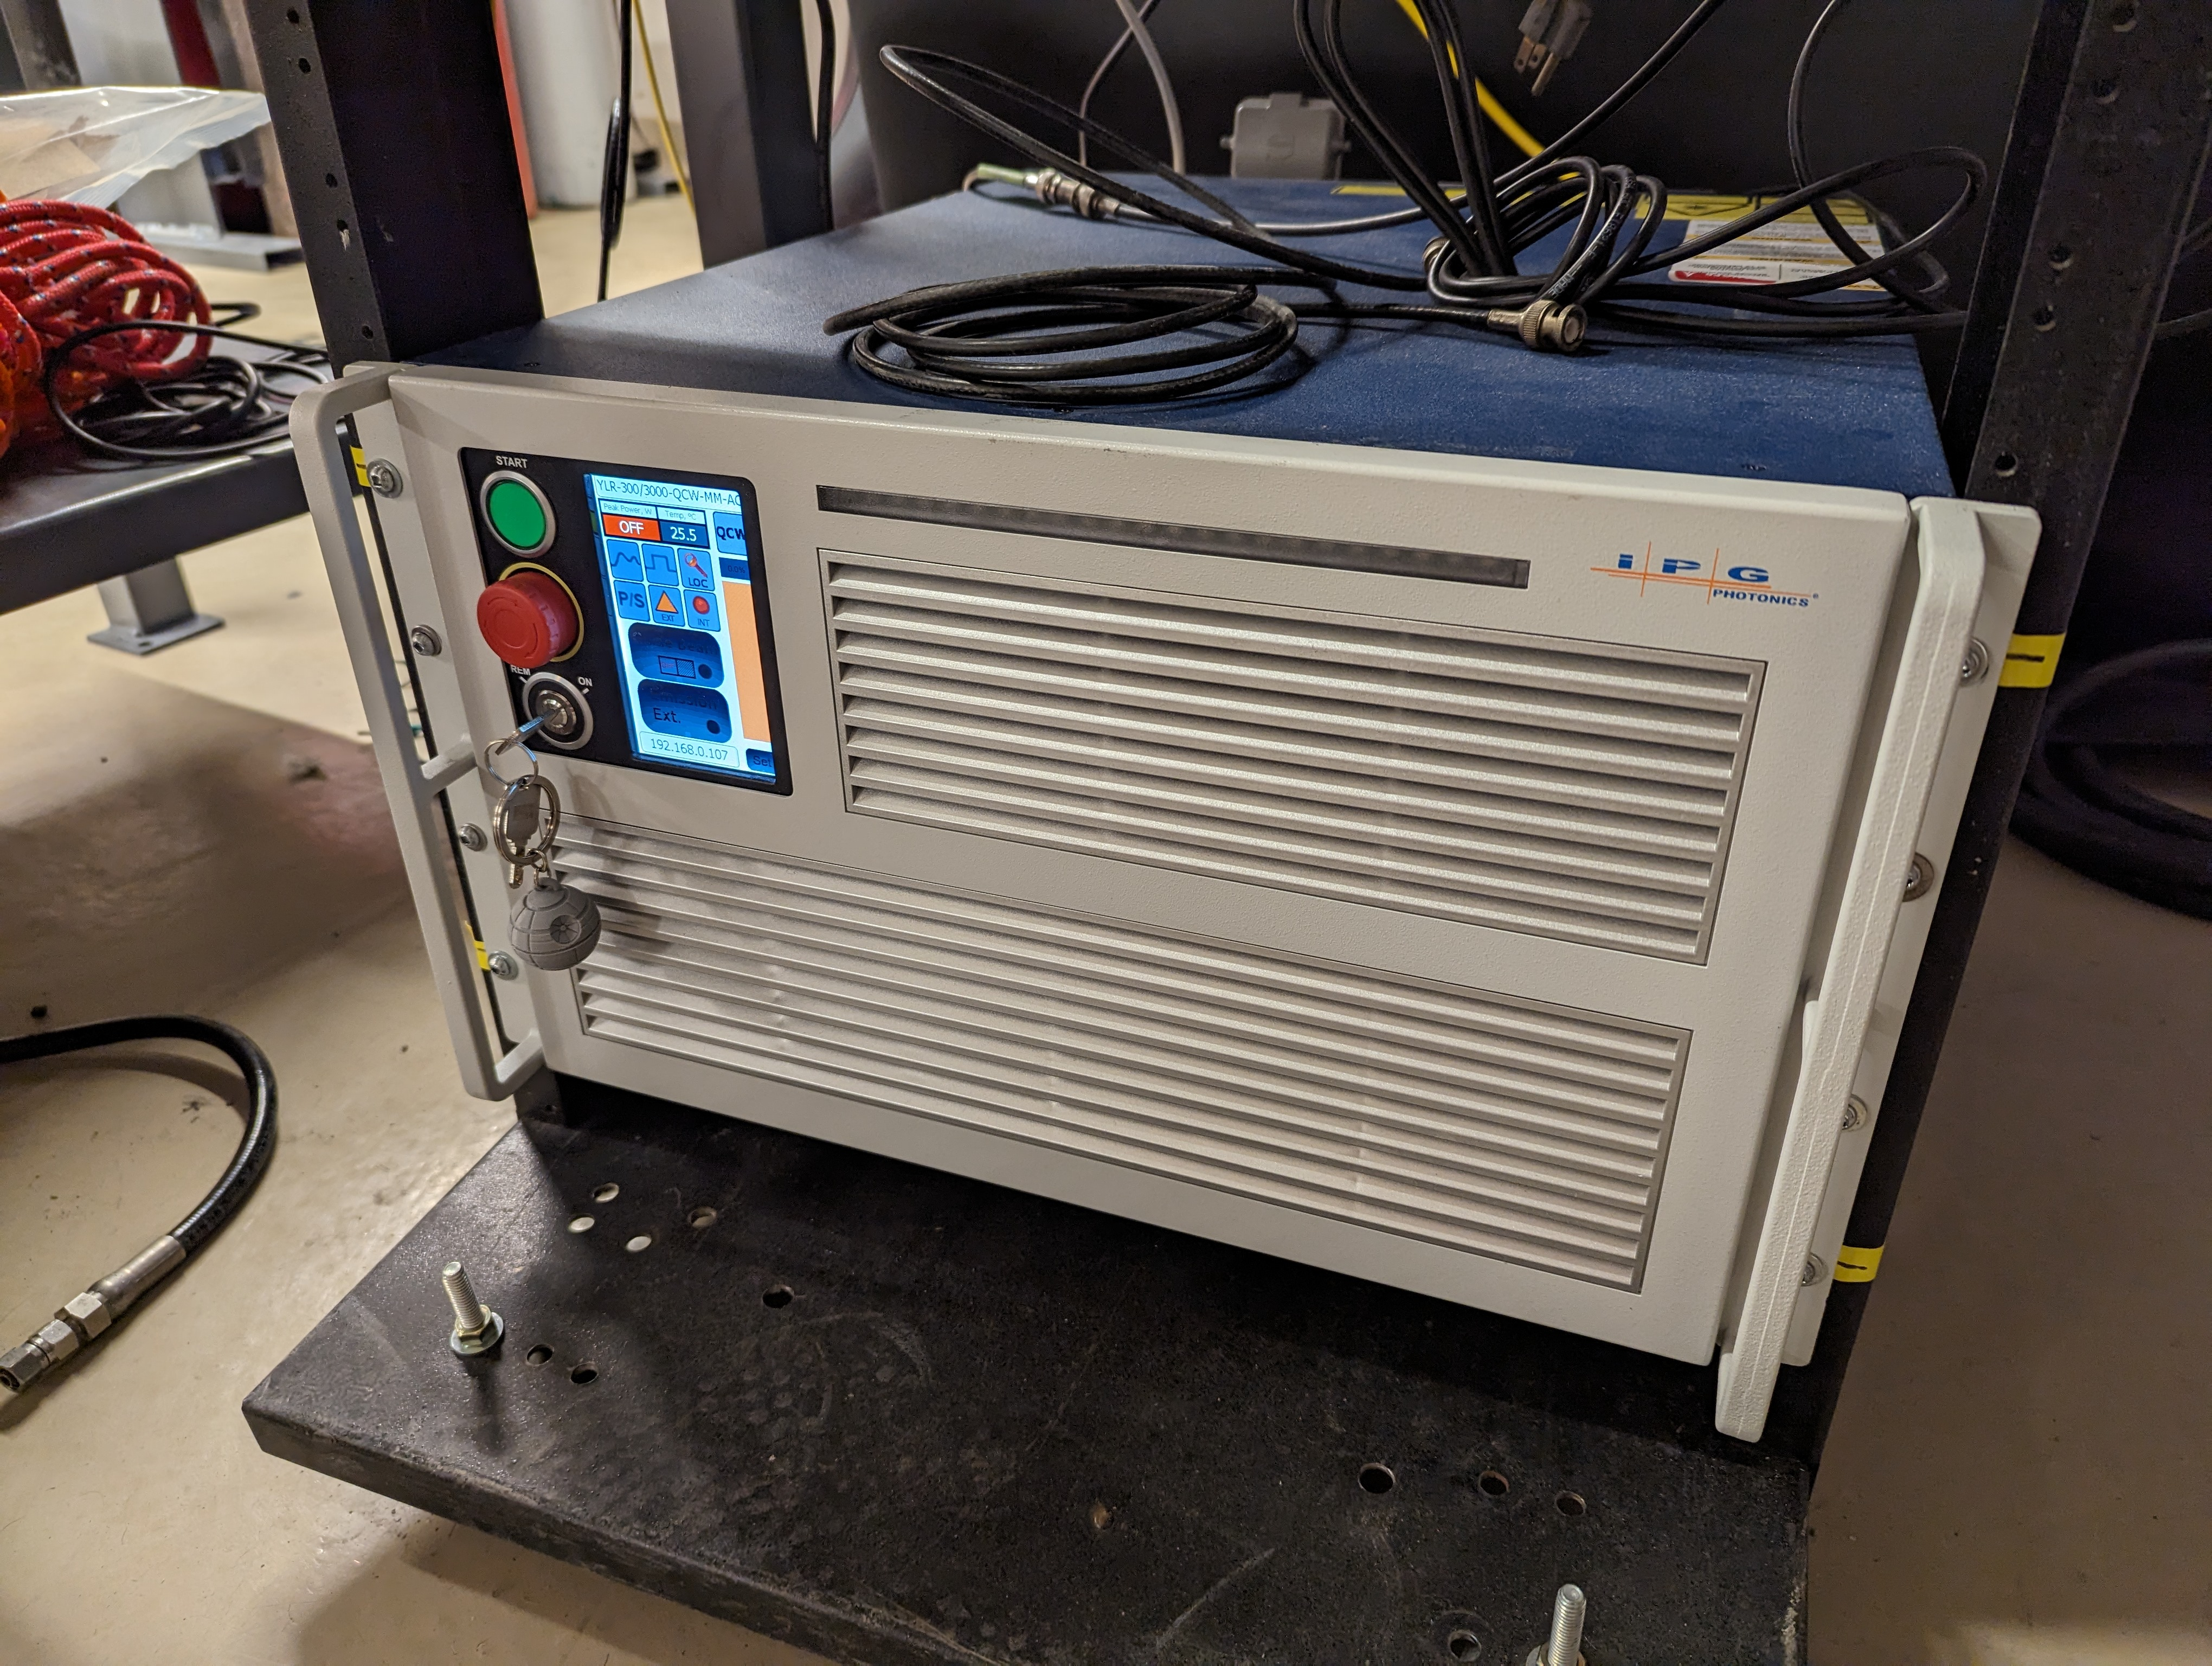
\includegraphics[height=2.6in]{assets/3 design/laser.jpg}
                    \caption{IPG Photonics YLR-300/3000-QCW-MM-AC Laser}
                    \label{fig:laser_laser}
                \end{subfigure}
                \hfill
                \begin{subfigure}[t]{0.35\textwidth}
                    \centering
                    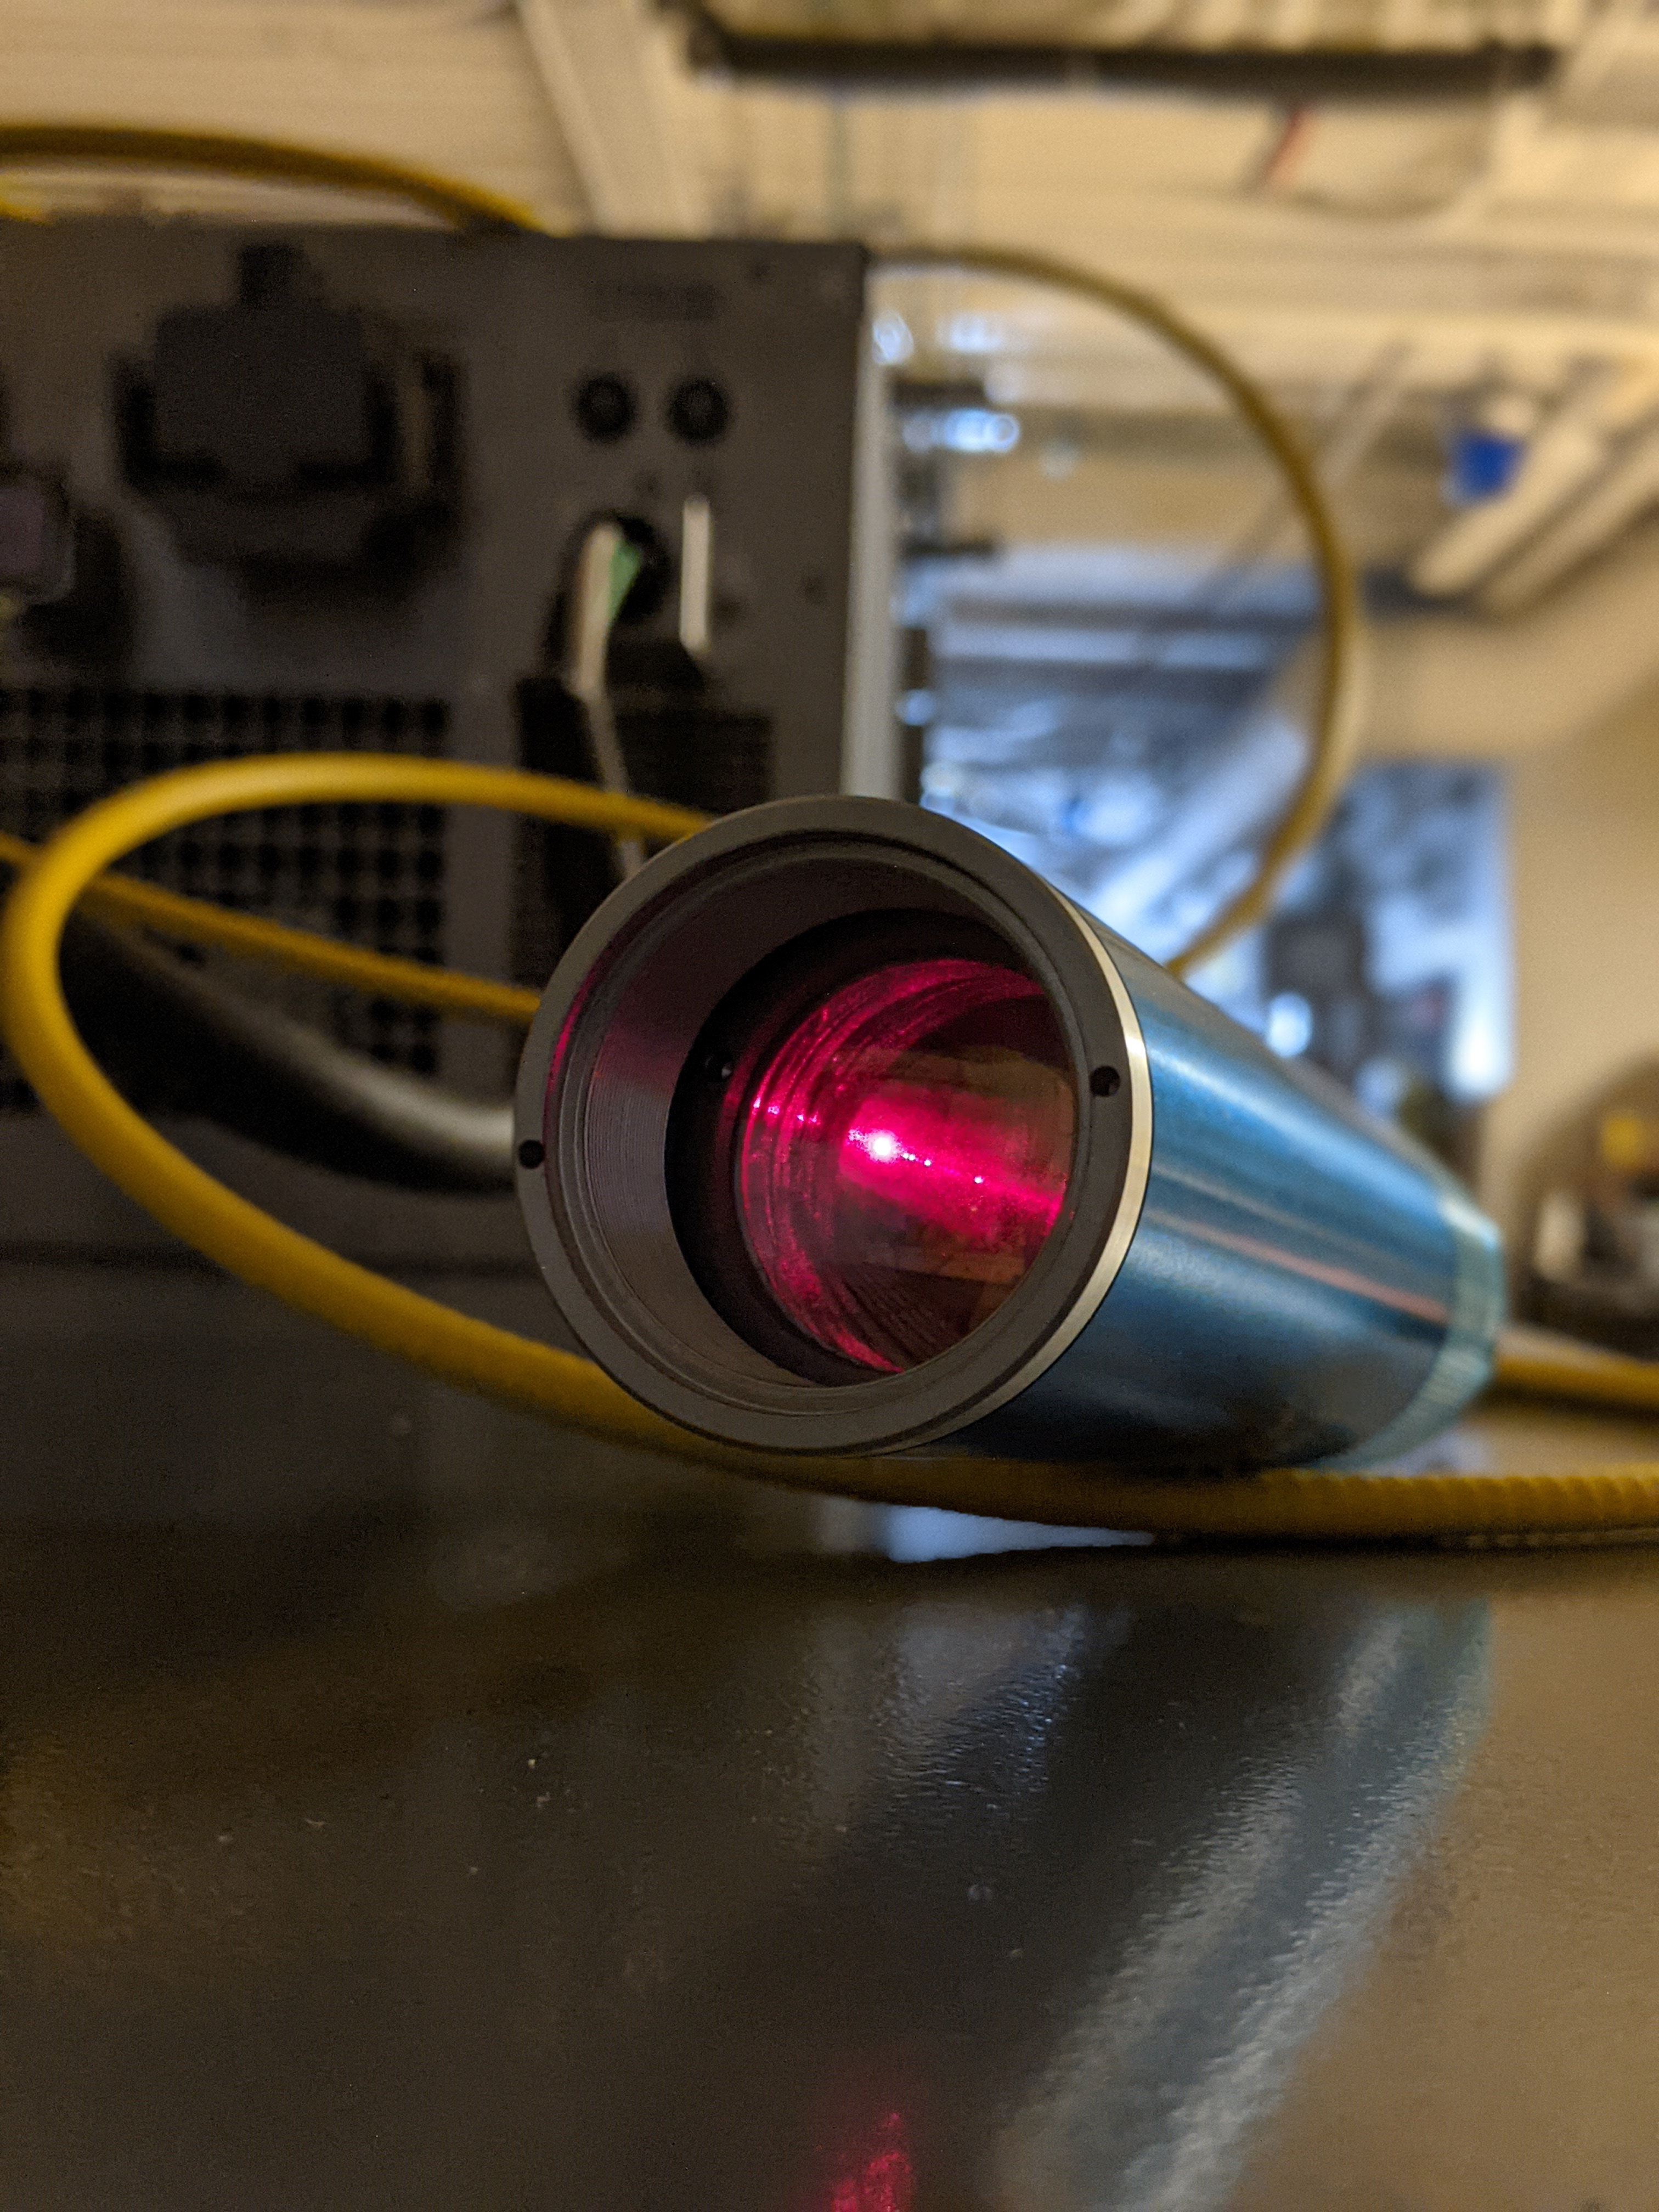
\includegraphics[height=2.6in]{assets/3 design/collimator_r.jpg}
                    \caption{Laser collimator head}
                    \label{fig:laser_collimator}
                \end{subfigure}
                \caption{Laser system used for this project}
                \label{fig:laser}
            \end{figure}

        \subsection{Instrumentation}
            The 10~ms experimental timescale meant that most instruments used on this experiment were selected based on their ability to make measurements within 10~ms or a sampling rate of at least \qty{1}{kHz}, where applicable.    

            \subsubsection*{Laser power meter}
                A laser power and energy meter was required to determine what fraction of laser power was absorbed by the LSP. A UP55N-300F-H12 power and energy meter from Gentec-EO was procured for this project. This thermopile power meter is rated for a maximum average power of 300~W and a maximum average power density of \qty{45}{kW.cm^{-2}}. These specifications\footnote{Its average power rating may be lower than the laser's peak power, but the pulsed mode allows for enough time for the power meter to cool down between pulses}, along with its ability to function as both a continuous power meter and a pulse energy meter, made it an excellent match for the IPG laser system. A selection of its nominal specifications can be found in \autoref{tab:laserPM_spec} and its calibration report can be found in \autoref{chp:app_calibration} page \pageref*{ds:laserPM}. Although the \num{3}-\unit{s}rise time appears to disqualify this power meter for pulsed experiments, using the power meter's pulse energy measurement mode bypasses this limitation. 

                \begin{table}[h]
                    \centering
                    \caption{Summary of nominal laser power meter specifications}
                    \label{tab:laserPM_spec}
                    \begin{tabular}{@{}lrl@{}}
                        \toprule
                        Parameter            & Quantity & Unit \\ \midrule
                        Calibrated Spectral Range     & 248--2100         & nm            \\
                        Maximum Average Power         & 300               & W             \\
                        Maximum Average Power Density & 45                & \unit{kW.cm^{-2}}             \\
                        Rise Time (0--95\%)          & 3                 & s            \\
                        Aperture Diameter             & 55                & mm           \\ 
                        Calibration Uncertainty       & 2.5               & \% \\
                        \bottomrule
                        \end{tabular}
                \end{table}

            \subsubsection*{High-speed camera}
                High-speed footage of the experiment was deemed necessary to study the behavior of LSP and determine some of its basic properties, such as dimensions, growth rate, and brightness. This was also the primary method to confirm successful LSP ignition. The camera used was a Photron FASTCAM SA5, capable of recording at up to 7000~fps at its full 1024$\times$1024~pixel resolution, and up to 775~000~fps when cropping the sensor. Most footage was recorded at 10~000~fps, providing sufficient temporal resolution while maintaining a relatively large field of view, which was necessary to capture the entirety of the plasma.

                The use of a high-power laser and the ignition of a plasma (bright source of UV) in the vicinity of this camera was concerning regarding potential damage to the camera sensor. Such damage would result in a lengthy, expensive repair procedure (or complete replacement), and interrupt or hinder not only this experiment, but several other concurrent projects in the lab, as this camera was shared across experiments. Several risk mitigation measures were put in place to minimize the likelihood of serious sensor damage:
                \begin{itemize}
                    \item The strategic use of aluminum safety screens to block the path of laser reflection
                    \item The use of a variable neutral-density filter capable of reducing incoming light intensity by a factor of 2000
                    \item The use of a UV-IR cut filter, reducing the intensity of radiation below 390~nm and above 700~nm by a factor of 100
                \end{itemize}
                Both filters were 58-mm-diameter commercial-grade photography filters fitted on a SIGMA 70-300~mm F4-5.6 DG MACRO zoom lens. 

                

            \subsubsection*{Pressure transducer} \label{sec:design_pressuresensor}
                While simple pressure gauges were sufficient for experiment set-up, pressure data with high temporal resolution was also of interest to study the effect of LSP ignition on the gas pressure, potentially using it as a proxy for temperature change and heat deposition within the test section. PCB Piezotronics 113B28 pressure transducers were sourced within the laboratory. Such transducers are used to detect changes from an initial pressure. With a rise time of less than \qty{1}{\um}\added{, a usable frequency range of more than \qty{100}{kHz}, }and a nominal sensitivity of \qty{14.5}{mV.kPa^{-1}}, these sensors are well suited to detect rapid and minute changes in pressure that would be expected in this experiment. The transducer's calibration report can be found in \autoref{chp:app_calibration} page \pageref*{ds:pcbPressure}.

                A possible concern regarding pressure from a safety, design, and measurement standpoint is whether the pressure rise resulting from heat deposition would exceed the measurement range of the transducer and/or the design pressures of the test section. The maximum possible pressure rise can be calculated assuming complete deposition of a laser pulse energy (\qty{30.8}{J}) into the working gas as heat. With the test section parameters seen in \autoref{sec:design_testSection} and \autoref{chp:app_CavitatorDrawings}, the maximum expected pressure rise is \qty{37.5}{kPa}, less than 2\% of the maximum design pressure, and equivalent to a \num{0.56}-\unit{V} rise from the pressure transducer, well within its design range\added{ of \qty{5}{V} (\qty{344.7}{kPa})}.

            \subsubsection*{Spectrometer}
                Spectrometry was identified as one of the primary methods to determine the LSP temperature. Indeed, the high expected plasma temperature (above \qty{10000}{K}) and the timescale of the event ($\sim$10~ms) meant that most intrusive methods (and some non-intrusive methods such as infrared thermometers) were inadequate.

                Spectrometry is commonly used in neighboring McGill laboratories studying combustion and metal fuels, so a portable USB spectrometer was easily sourced for this experiment. The Ocean Optics (now Ocean Insight) USB4000 \cite{oceanopticsUSB4000FiberOptic2008} is a compact spectrometer with a measurement range of \qtyrange{200}{1100}{nm} and a minimum integration time (analogous to exposure time for a camera) of 3.8~ms. \added{Although this may not satisfy the sampling rate requirement stated at the start of this section, this was deemed sufficient as determining the temporal change in LSP temperature was not within the scope of the experiment.} Varying diameters of fiber optics were tested to determine the optimal fiber size: as this spectrometer was used without a\replaced{n aperture slit}{ diffraction grating}, the fiber core diameter \replaced{affected}{determined} the spectral resolution\replaced{. S}{, with s}maller apertures \added{cast a wider beam on the diffraction grating, illuminating a greater number of grooves and thus} providing finer wavelength separation~\cite{naveDiffractionGratingResolution2000}\deleted{, at the cost of reduced brightness}. 
                
                \replaced{The use of smaller entrance apertures comes at the cost of reducing the signal strength (i.e., brightness), but}{However,} the LSP brightness was found to be sufficient to provide a clear spectrum even with the narrowest available 10-\unit{\um} fiber. The spectrometer was calibrated using an Ocean Optics HG-1 Mercury Argon Light Source for wavelength calibration (ensuring the sensor's pixels match to the correct wavelength), and an Ocean Insight HL-2000 Halogen Light Source for relative intensity calibration (correcting for uneven sensitivity across the captured spectrum).

    \section{Design process}
        The design of custom hardware was necessary for this experiment. This included a pressurized test section and an ignition system. As mentioned in \autoref{sec:design_ots}, a thrust stand was also needed, but its design was delegated to a team of students assisting in the project. These design activities, along with the thrust stand requirements given to the students, will be documented here.

        \subsection{Test section} \label{sec:design_testSection}
            The requirements for the Laser-Thermal Thruster Laboratory Model (LTTLM) are listed in \autoref{tab:lttmReq}. In summary, the thruster model should be a pressurized vessel featuring one or more windows to allow laser input and optical viewing of the LSP. Furthermore, this vessel should allow the integration of various instrumentation systems. The design and manufacture of such a vessel would have required a significant amount of time, so the alternative of re-purposing hardware from a different project was considered first. This hardware's specifications could be compared to the requirements, and modifications could be made if necessary.

            \begin{table}[h]
                \renewcommand{\arraystretch}{1.3}
                \centering
                \caption[Top-level design requirements for the LTP laboratory model]{Top-level design requirements for the LTP laboratory model (the ``thruster'')}
                \label{tab:lttmReq}
                \begin{tabular}{l>{\raggedright}p{0.4\textwidth}p{0.4\textwidth}<{\raggedright}}
                    \toprule
                    Identifier  & Requirement   & Rationale \\
                    \midrule
                    LTTLM-1     & The thruster shall operate at a maximum laser power of \qty{3}{kW} at a wavelength of \qty{1070}{nm}    & This is the laser system made available for this experiment \\
                    LTTLM-2     & The thruster shall operate using gaseous argon at room temperature as a propellant & The past experiments used for comparison also used argon \\
                    LTTLM-3     & The thruster shall operate at a maximum design pressure of 2~\unit{MPa} & This should allow the generation of LSP even in continuous-wave laser modes \\
                    LTTLM-4     & The thruster shall allow visible observation of the LSP in the thrust chamber & This enables high-speed imaging of the plasma and the remote measurement of its temperature \\
                    LTTLM-5     & The thruster shall provide\added{ interfaces to allow for measuring} chamber pressure and gas temperature \deleted{data}  & This permits the estimation of stagnation conditions for the heated propellant \\
                    LTTLM-6     & The thruster shall \replaced{provide interfaces to allow for measuring}{allow the measurement of} absorbed laser power   & This is one of the major energy losses to be determined \\
                    \added{LTTLM-7}     & \added{The thruster shall have a structural safety factor of 10}  & \added{This provides an adequate safety margin for operating the thruster} \\
                    \bottomrule
                \end{tabular}
            \end{table}

            Coincidentally, \textcite{kokkalisOnsetCavitationDynamically2023} at the neighboring McGill Fluid Dynamics Lab (FDL) was undertaking research into cavitation effects within piston-cylinder assemblies. His apparatus included cylindrical sections designed to withstand high dynamic pressures encountered in their experiments, and featured windows or transparent walls to track the onset of cavitation with high-speed cameras. The design was modular, allowing the installation of various endcaps with different functions. This theoretically fulfilled requirements LTTLM\nobreakdash-2 to LTTLM\nobreakdash-4. One particular test section (pictured in \autoref{fig:cavitation}, detailed drawings can be found in \autoref{chp:app_CavitatorDrawings}) had been fabricated with a set of instrumentation ports and polycarbonate windows spanning the length of the cylinder. This test section had been tested in a few experiments examining dynamic cavitation in water but was found to be inadequate, as gaps around the ports and windows were sources of parasitic cavitation.

            \begin{figure}[h]
                \centering
                \begin{subfigure}[t]{0.46\textwidth}
                    \centering
                    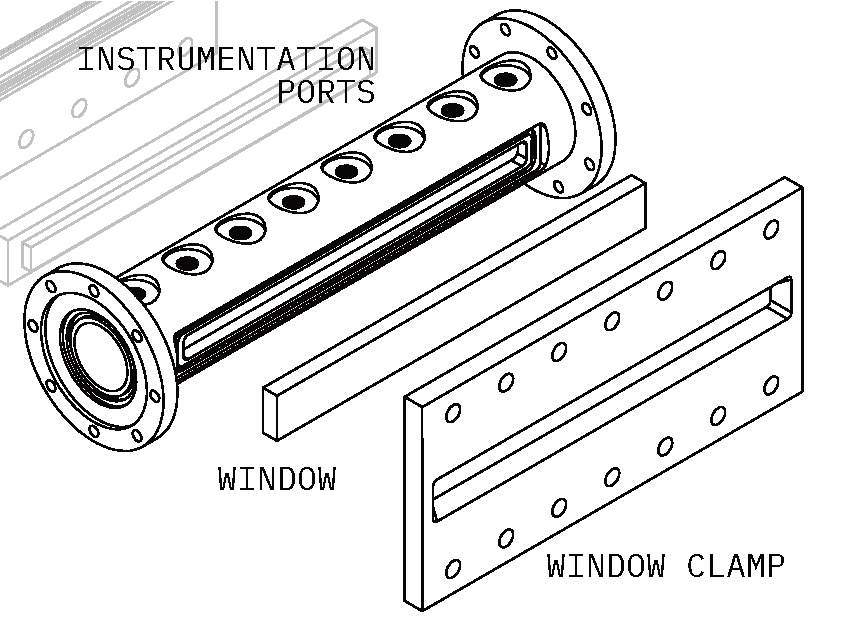
\includegraphics[width=\textwidth]{assets/3 design/cavitatorDrawing}
                    \caption{Assembly schematic}
                    \label{fig:cavitation_schematic}
                \end{subfigure}
                \hfill
                \begin{subfigure}[t]{0.49\textwidth}
                    \centering
                    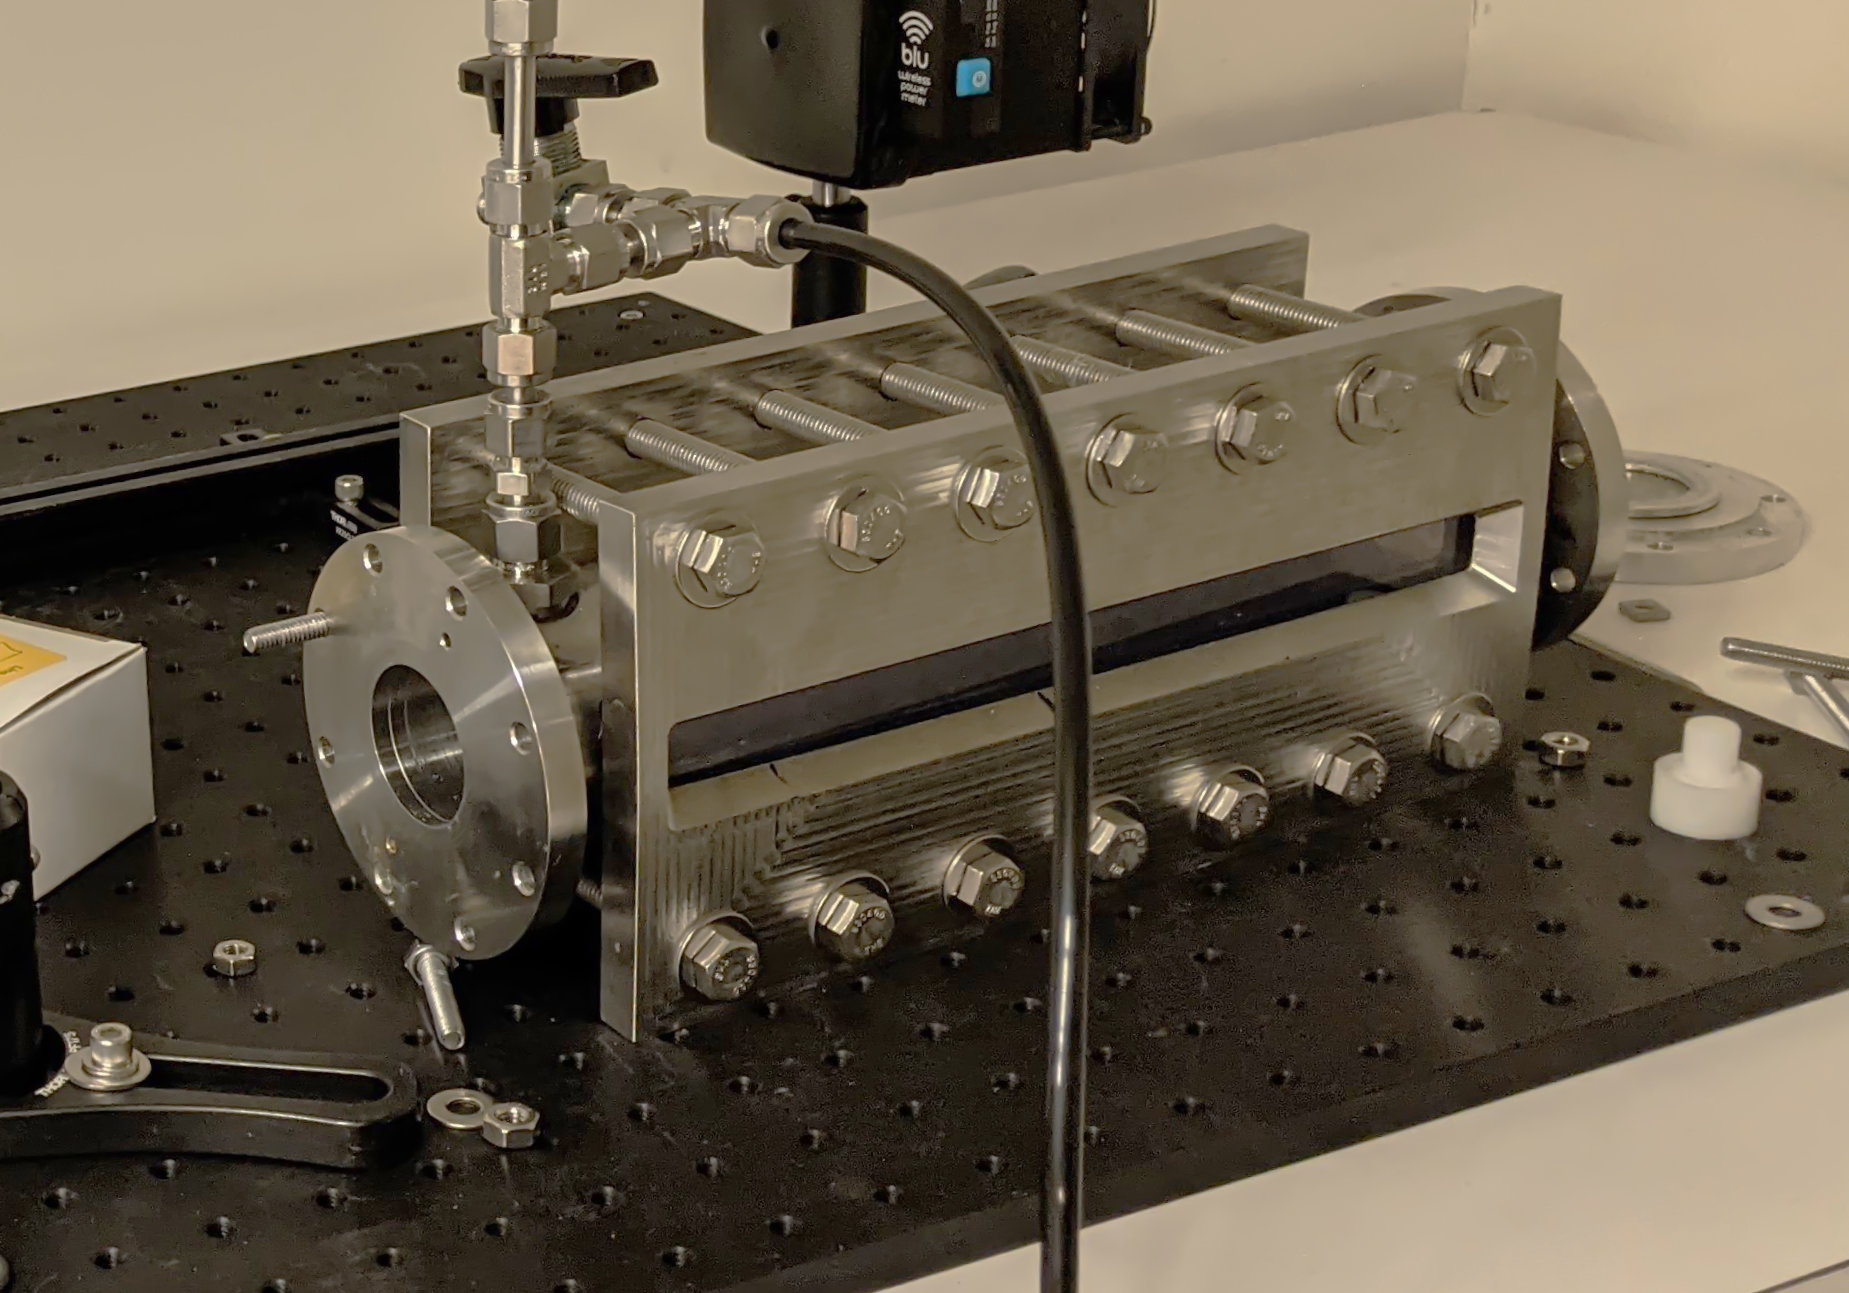
\includegraphics[width=\textwidth]{assets/3 design/cavitationSection.jpg}
                    \caption{Photograph of the test section fitted with a gas feed line}
                    \label{fig:cavitation_photo}
                \end{subfigure}
                \begin{subfigure}[t]{\textwidth}
                    \centering
                    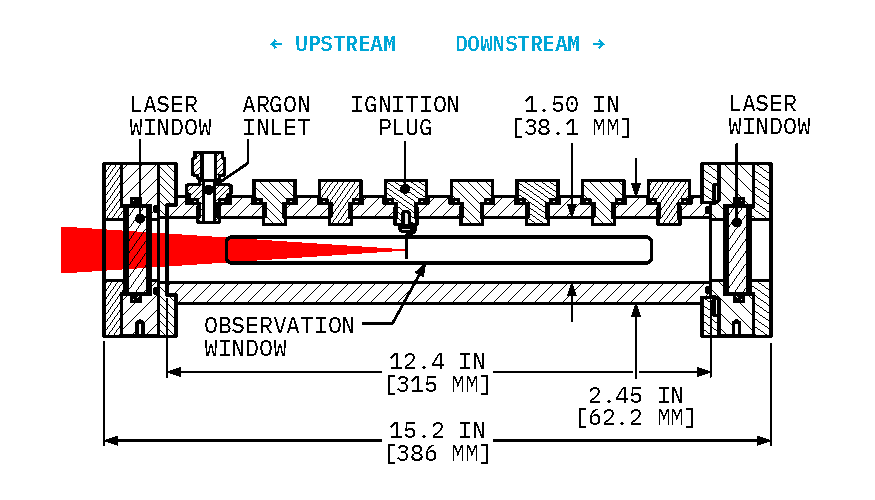
\includegraphics[]{assets/3 design/testsection_layout.pdf}
                    \caption{Basic dimensions. Detailed drawings available in \autoref{chp:app_CavitatorDrawings} and \autoref{chp:app_lwmDrawings}}
                    \label{fig:cavitation_dimensions}
                \end{subfigure}
                \caption{Laser ionization test section}
                \label{fig:cavitation}
            \end{figure}

            As seen in \autoref{tab:lttmReq_partialVerif}, this apparatus was verified against the requirements set in \autoref{tab:lttmReq} to determine what retrofitting activities would be needed to use it as an LTP thruster model. It was found that very little retrofitting work was required in order to use it as an LSP generator: special instrument plugs could be created, and special laser window endcaps were needed to seal the apparatus while allowing the laser to enter the test section. To operate the system as a thruster, an existing blank endcap could be modified to accept small nozzles.\added{ The apparatus was designed to withstand much greater pressures than the 20-bar design pressure, was tested to withstand this pressure, and a thick-walled pressure vessel calculation showed it had a hoop-stress safety factor of 50 for this application.} Finally, as spectrometry was planned to be used for plasma temperature determination, the polycarbonate side windows would have to be exchanged for UV-grade quartz windows, which would allow a broader spectrum of radiation to pass through.
        
            \begin{table}[h]
                \renewcommand{\arraystretch}{1.3}
                \centering
                \caption{Verification of LTTLM requirements for the cavitation apparatus}
                \label{tab:lttmReq_partialVerif}
                \begin{tabular}{l>{\raggedright}p{0.53\textwidth}p{0.27\textwidth}<{\raggedright}}
                    \toprule
                    Identifier & Requirement                                                                   & Status                   \\ \midrule
                    LTTLM-1             & The thruster shall operate at a maximum laser power of \qty{3}{kW} at a wavelength of \qty{1070}{nm} & Requires laser windows            \\
                    LTTLM-2             & The thruster shall operate using gaseous argon at room temperature as a propellant     & Fulfilled                         \\
                    LTTLM-3             & The thruster shall operate at a maximum design pressure of 2 MPa                       & Fulfilled                         \\
                    LTTLM-4             & The thruster shall allow visible observation of the LSP in the thrust chamber          & Fulfilled                         \\
                    LTTLM-5             & The thruster shall provide\added{ interfaces to allow for measuring} chamber pressure and gas temperature \deleted{data}                   & Requires special instrument plugs \\
                    LTTLM-6             & The thruster shall \replaced{provide interfaces to allow for measuring}{allow the measurement of} absorbed laser power                       & Requires laser windows            \\ 
                    \added{LTTLM-7}     & \added{The thruster shall have a structural safety factor of 10}  & \added{Fulfilled}\\
                    \bottomrule
                \end{tabular}
            \end{table}
            
            However, using this test section would not come without a set of drawbacks. Its original intent made it unoptimized to work as a laser-thermal thruster model for the following reasons:
            \begin{enumerate}
                \item Although its thick stainless-steel construction made it very safe for the operating pressures of the project, it also made it heavy. The superfluous mass would make frictional loads on a thrust bench far more significant than for a custom-designed, lightweight thruster model.
                \item Its length forces the use of long focal-length lenses to focus the laser into the test section. Such long lenses would create a high {\itshape f}-number beam, which could affect how easily a stable LSP could be achieved, as discussed in \autoref{sec:background_lsp}. While shorter lenses would still be able to focus the laser into the chamber, the beam past the focal point would diverge quickly and hit the test section walls, affecting laser absorption measurements at best, or damaging experimental apparatus at worst.
                \item Instrumentation ports are available only on one side of the cylinder. The lack of opposing ports constrains the design of certain ignition methods, such as spark igniters.
            \end{enumerate}

            The alternative was to work on a clean-sheet design that would perfectly satisfy the requirements set in \autoref{tab:lttmReq}, without the drawbacks of the existing apparatus listed above. While this may have avoided many difficulties encountered later in this project, opting for a custom design would have introduced significant risks in terms of timeline, compounded by the many uncertainties surrounding the operation of an LSP generator/LTP thruster. In order to quickly move forward with the project, it was decided to retrofit the existing cavitation apparatus into an LSP generator. It was reasoned that the lessons learned in attempting experiments with an unoptimized system would still be valuable to document and would be very effective in informing the design of a custom thruster laboratory model.

        \subsection{Laser window mount} \label{sec:design_lwm}
            The first and most important retrofitting task was the implementation of windows allowing the laser to enter the test section, then exit it, with minimal power losses. In terms of methodology, significant power losses would be acceptable as long as they are measurable and consistent, such that they can be accounted for. However, minimizing them is beneficial to allow the complete use of the laser's power range. As anti-reflection coated optics could readily be found with less than 1\% power losses, this was deemed as an acceptable threshold.

            Three major requirements thus drove the laser window design:
            \begin{enumerate}
                \item The window shall transmit at least 99\% of the incident laser power. \emph{Rationale:} this maximizes the available laser power within the test section.
                \item The window shall seal the test section at 20~bar and remain structurally sound. \emph{Rationale:} this directly derives from requirement LTTLM-3.
                \item \added{The window shall have a structural safety factor of 10. \emph{Rationale:} this directly derives from requirement LTTLM-7.}
            \end{enumerate}

            Pressure vessel windows are often needed in the IFERG---the group has thus acquired useful experience on their design, adopting design guidelines from the \textcite{brookhavennationallaboratoryGuideGlassPlastic2005}. In summary, these guidelines provide design formulas, empirically derived properties, and tried-and-tested designs for various applications. The window mount follows the ``free edges'' design (Figure 14 in \cite{brookhavennationallaboratoryGuideGlassPlastic2005}), deemed most appropriate for this application, and having been successfully implemented\footnote{A former laboratory member consulted on this design problem stated: ``Every time I did not follow this guide to the letter, it failed.''} in past experiments. In this design, a peripheral o-ring provides a reliable seal, while two rubber or Teflon gaskets support the window and prevent its edges from touching the metal walls. This is the critical design criterion for pressure windows: although glass and crystals often exhibit excellent tensile strength, their brittleness makes them susceptible to localized stress concentrations which ultimately are the source of failure. This occurs at glass-metal contact points, so pressure window designs focus on preventing these contacts by minimizing strain and introducing soft interfaces such as Teflon or rubber gaskets.

            The calculation procedure described in \cite{brookhavennationallaboratoryGuideGlassPlastic2005} for elliptical windows was used to size an appropriate window based on different materials and suppliers. Sapphire, borosilicate glass (N-BK7), and quartz were considered as potential materials. Strict application of the guide's mandated safety factor of 10 and the use of the full test section internal diameter (\qty{38.1}{mm} or 1.5~in) as the aperture size led to window dimensions that could not be sourced from off-the-shelf suppliers. To reduce costs and facilitate supply, a compromise was reached by reducing the effective aperture to 1.4~in (\qty{35.6}{mm}) to provide more support to the window while accepting a reduced safety factor of about 9.1. The resulting window is 12-mm-thick and \qty{50.8}{mm} in diameter for N-BK7 glass, which is supplied by Thorlabs as WG12012-C~\cite{thorlabsWG12012CO2NBK7}. Other suppliers either could not supply a window matching these specifications or did so for a much higher price. Likewise, other material choices resulted in window dimensions that could not be sourced off-the-shelf.

            Window mounts (pictured in \autoref{fig:windowMount}) were then designed to interface with the existing apparatus, following the ``free edges'' design. As the existing apparatus had no mounting arrangements, the window mounts also featured a tapped hole allowing the mounting of optical posts (as seen in \autoref{fig:windowMount_empty}) to the assembled test section. This permitted its integration with an optical table system, greatly facilitating experimental setup. Complete drawings for the window mounts can be found in \autoref{chp:app_lwmDrawings}.

            \begin{figure}[h]
                \centering
                \begin{subfigure}[t]{0.48\textwidth}
                    \centering
                    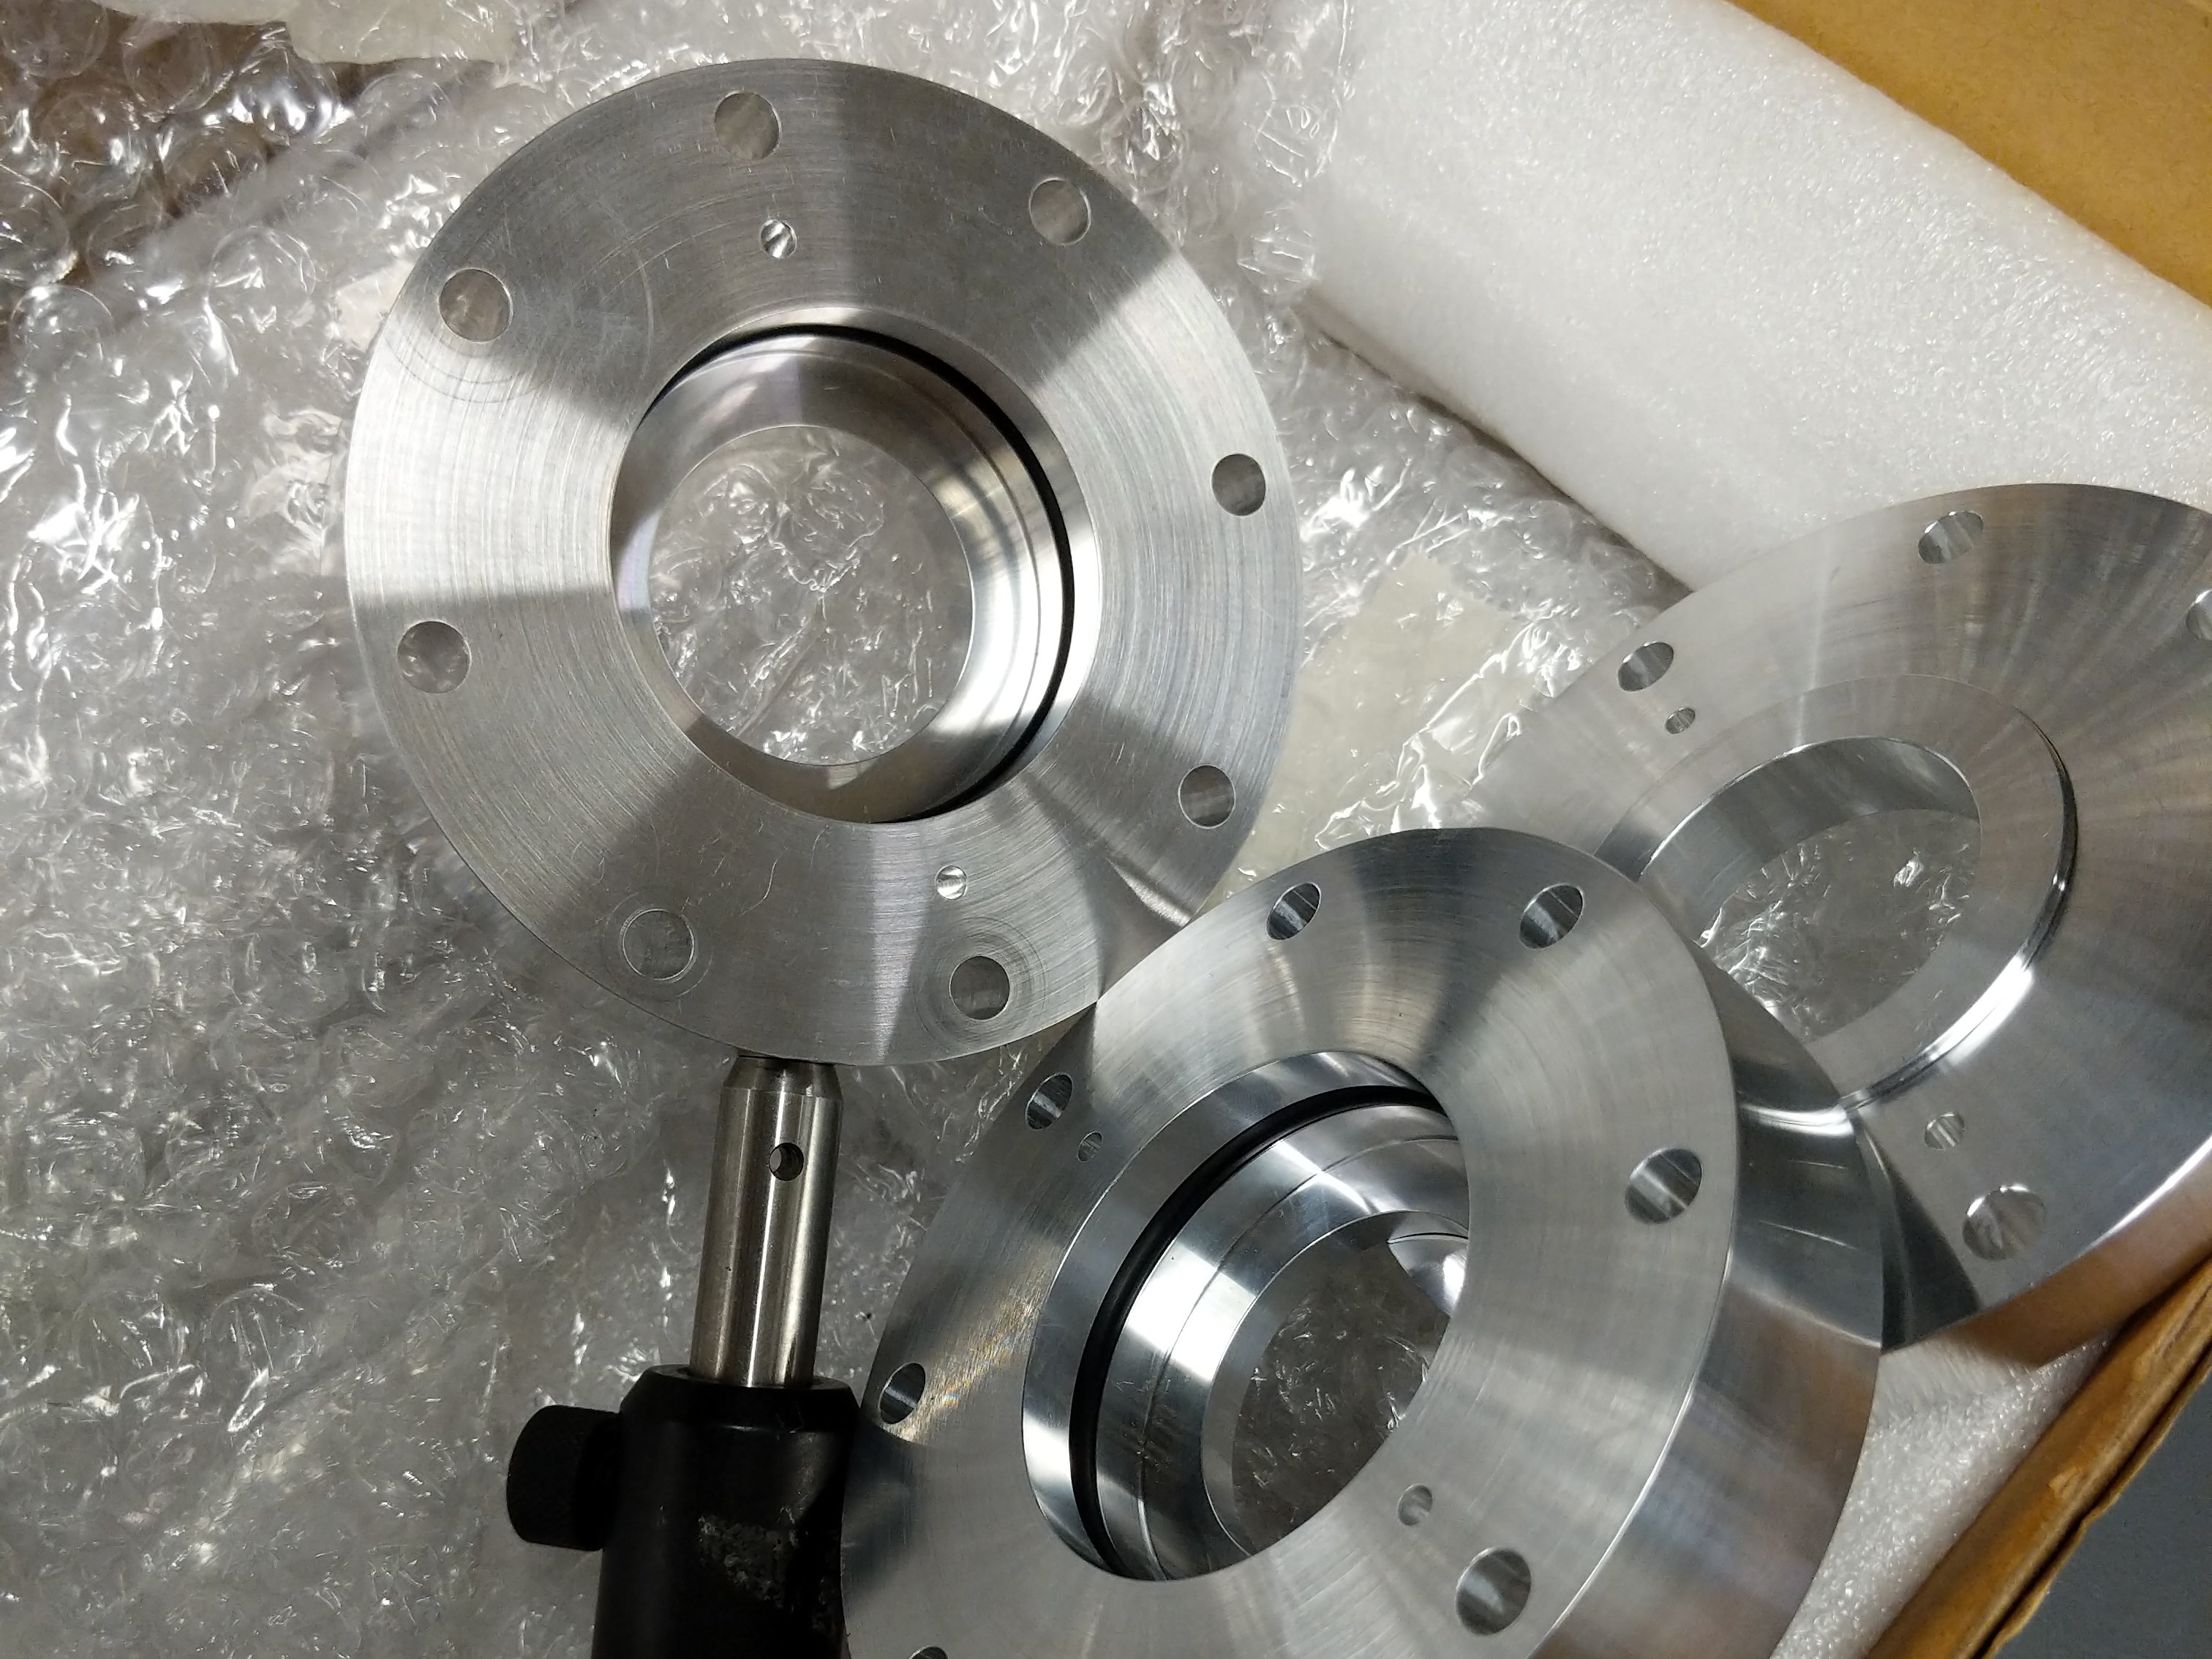
\includegraphics[width=\textwidth]{assets/3 design/windowMount_empty.jpg}
                    \caption{O-ring installed and mounted on optical post}
                    \label{fig:windowMount_empty}
                \end{subfigure}
                \hfill
                \begin{subfigure}[t]{0.48\textwidth}
                    \centering
                    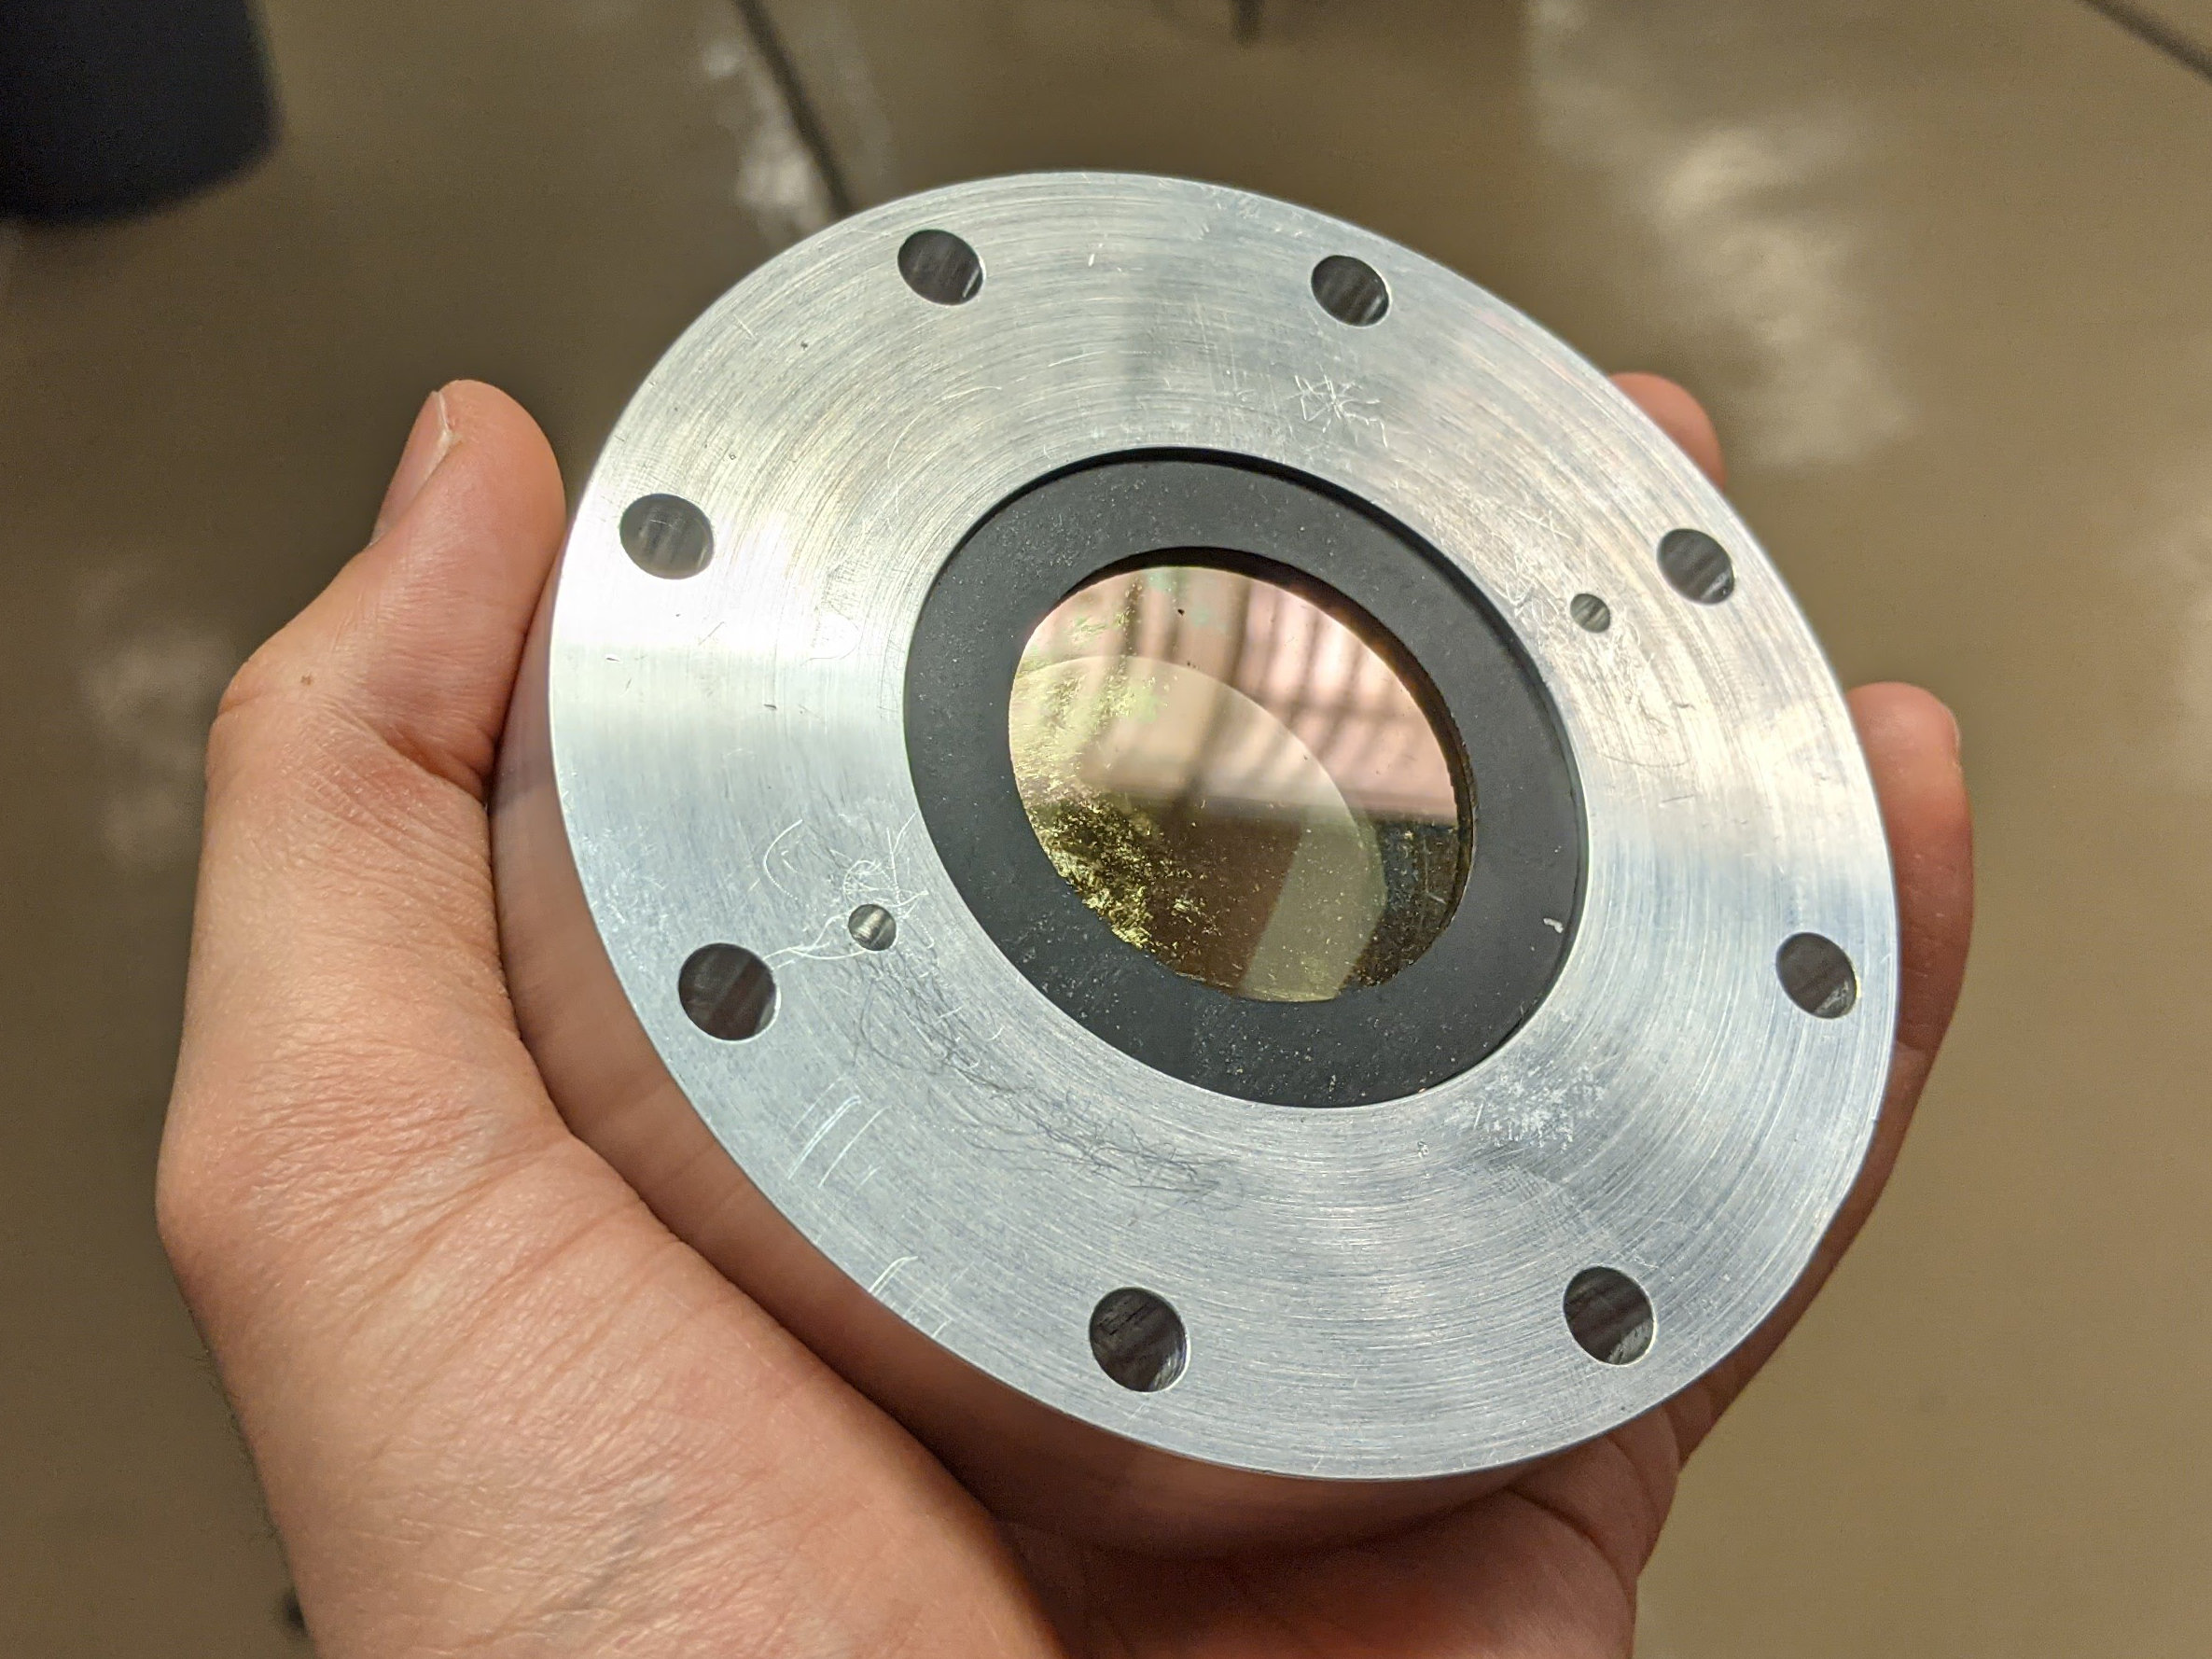
\includegraphics[width=\textwidth]{assets/3 design/windowMount_installed.jpg}
                    \caption{Window installed in mount with gasket}
                    \label{fig:windowMount_installed}
                \end{subfigure}
                \caption{Laser window mounts}
                \label{fig:windowMount}
            \end{figure}

        \subsection{UV-grade side windows}
            The windows installed on the existing cavitation apparatus were bonded acrylic and polycarbonate. While this was sufficient for observation in the visible spectrum, these materials are less suitable to perform spectroscopy, which would be an integral part of the instrumentation used for the project. Data gathered by \textcite{zimakovInteractionNearIRLaser2016,luCharacteristicDiagnosticsLaserStabilized2022} suggest significant radiation emission both in the near ultraviolet and near infrared. Polycarbonate and acrylic both feature a sharp drop in transmission between 400 and 450~\unit{nm}, along with irregular (although admittedly high) transmission in the near-IR~\cite{gsplasticopticsTransmissionCurvesOptics}. To ensure a complete picture of the plasma's radiation emission was captured, the decision was made to replace these plastic windows with UV-grade fused silica (JGS1). As seen in \autoref{fig:jgs1}, this material features a relatively uniform transmission profile from \qtyrange{210}{1000}{nm}. An added benefit of the new windows was greater optical clarity in the visible spectrum as well. Windows matching the geometry of the polycarbonate windows were ordered from Dalian Unique Optics Co., Ltd. in China. A set of gaskets cut out of Buna-N rubber were used to seal and protect the window, as it is subject to the same failure modes discussed in \autoref{sec:design_lwm}.

            \begin{figure}[h]
                \centering
                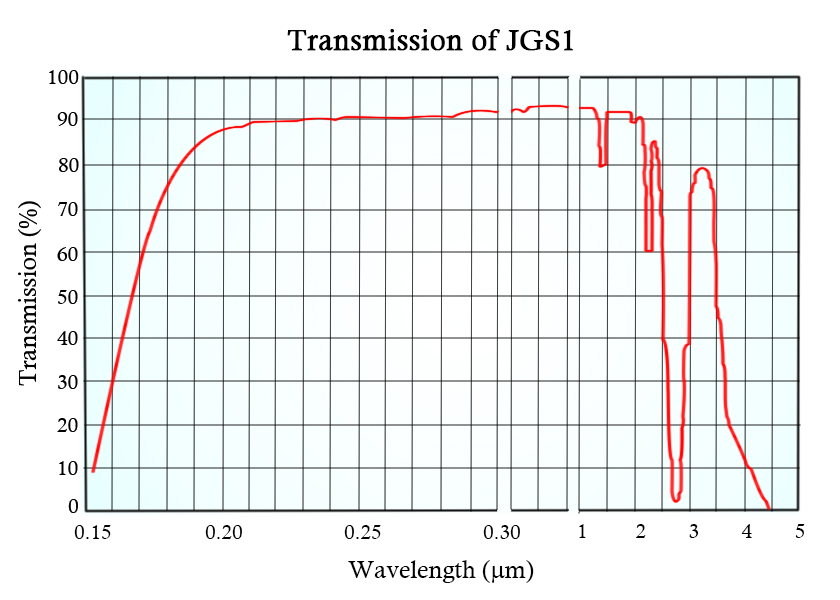
\includegraphics[width=0.85\textwidth, clip, trim=0 0 0 15pt]{assets/3 design/jgs1_transmission.jpg}
                \caption[Transmission profile of JGS1 fused silica]{Transmission profile of JGS1 fused silica~\cite{shalomeoJGS1}}
                \label{fig:jgs1}
            \end{figure}

        \subsection{Spark-ignition system} \label{sec:sparkignition}
            As seen in \autoref{sec:background_exp}, several methods were devised to ignite LSP, i.e. create a seed plasma that could initiate the inverse bremsstrahlung laser absorption mechanism. These include:
            \begin{itemize}
                \item Inducing a plasma using a separate high-power laser pulse
                \item Focusing the laser onto a solid tungsten or titanium target, releasing an electron cloud by thermionic emission (\textcite{schwartzLasersustainedGasPlasmas1989}) that could initiate LSP
                \item Focusing the laser onto an electrical arc discharge across two electrodes
            \end{itemize}
            An ignition mechanism was selected based on available resources and experimental requirements, namely:
            \begin{enumerate}
                \item The ignition system shall not impede the measurement of absorbed laser power by the plasma. \emph{Rationale:} derives directly from requirement LTTLM-6.
                \item The ignition system shall operate on a millisecond timescale. \emph{Rationale:} the laser pulse will be as short as 10~ms, so an ignition system should function within a couple of milliseconds or be capable of triggering with millisecond precision.
            \end{enumerate}
            The use of a separate high-power laser pulse to induce a seed plasma would likely fulfill both requirements, as this is a non-intrusive ignition method, and such lasers often operate with nanosecond pulses or shorter. However, this would require the purchase of a second laser system at a high cost and a long lead time, so this option was discarded. Solid metal targets offer an easy to implement, reliable, and affordable ignition solution, but was thought to be unable to fulfill the requirements listed above: Placing a solid target in the beam path would prevent the measurement of laser power exiting the plasma. While actuators could be used to remove the target, these would add complexity and likely be unable to operate within the desired timescale.

            This left spark ignition as the preferred solution: spark igniters are easily triggered with precision thanks to their fully electrical, solid-state operation, the lack of moving parts also facilitate sealing, and the electrode spacing can be controlled to avoid intersecting the laser beam path. Furthermore, such systems have been in use in various other projects in the laboratory, so this would build on past experience.

            Past work within the laboratory and the Thermodynamics and Combustion Group of Concordia University converged on a design based on the use of ``smart'' high-performance automotive ignition coils. Such coils are charged with a DC power supply and triggered based on a Transistor-to-Transistor Logic (TTL) signal, which can be generated by a wide variety of electronics, including precision digital delay generators commonly used in the laboratory. Reliable spark-igniter operation had previously been achieved with the AEM 30-2853 High Output Smart Coil. This coil can output a \num{40}-\unit{kV} voltage and a spark energy of up to \qty{103}{mJ}. Detailed specifications can be found in its instruction manual~\cite{aemperformanceelectronicsInstructionManual302853}.
            
            The spark-igniter circuit design (illustrated in \autoref{fig:spark_circuit}) was adapted and greatly simplified from previous implementations for other projects, as this experiment only required a single arc discharge at a time. Previous igniter designs featured control electronics to trigger a series of sparks---these electronics were discarded as they introduced complexity and unreliability for the benefit of flexibility that was not needed in this project. In this simplified design, the coil awaits a 3- to 9-ms-long 5-V gate signal to charge. This gate signal is generated directly by a delay generator that can be triggered manually or from an external signal. Once the gate signal ends, the coil releases its energy through the high voltage terminal at \qty{40}{kV}. This energy discharges across the spark plug's electrodes, creating a spark. The negative electrode is connected to the coil's spark ground (on pin 3), the test section body, and a real ground wire, to ensure that no residual voltage remains in the system.

            \begin{figure}[h]
                \centering
                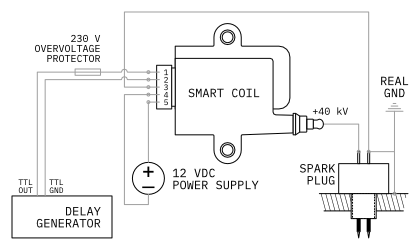
\includegraphics[]{assets/3 design/sparkIgniter}
                \caption[Spark-ignition circuit diagram]{Spark-ignition circuit diagram. Not pictured are various switches used to safely operate the system.}
                \label{fig:spark_circuit}
            \end{figure}

            \autoref{fig:spark_circuit} also depicts the custom spark plugs fabricated for this experiment: two holes were drilled in blank Delrin plugs, through which industrial steel sowing needles were driven. After bonding them to the plug body with epoxy and applying insulation, these plugs were fitted with wire terminals to connect to the smart coil. A notable difference in this design from past literature is the use of side-by-side electrodes instead of electrodes inserted at opposite ends and meeting in the middle. This was due to the absence of opposing ports on the test section. The drawback of this design is a greater likelihood of a spark forming somewhere other than between both needle tips, but the use of insulation mitigated this issue.

            Electrode spacing is a key design parameter for the custom spark plug. The discharge arc length $d$ is a function of the gas properties, pressure $p$, and applied voltage $V_\mathrm{B}$, as seen in \autoref{eq:paschen}:
            \begin{equation}
                V_\mathrm{B} = \frac{\mathsf{B} pd}{\ln{(\mathsf{A} pd)}-\ln{\left(\ln{\left(1+\frac{1}{\gamma_\mathrm{se}}\right)}\right)}}
                \label{eq:paschen}
            \end{equation}
            This is known as Paschen's law. The parameters $\mathsf{A}$ and $\mathsf{B}$ depend on the gas and are determined experimentally. The secondary-electron-emission coefficient $\gamma_\mathrm{se}$ is also different for each gas~\cite{liebermanPrinciplesPlasmaDischarges2005}. This equation can be solved (numerically) for the electrode distance required to arc at a certain voltage and pressure. This is shown in \autoref{fig:paschenPressure}, where the required voltage is plotted for the range of operating pressures planned for the experiment. A line is drawn at \qty{40}{kV} to represent the smart coil's output---in theory, as long as this line intersects all pressure curves, there exists an electrode distance at which the spark plug will successfully arc. The values used for this model are as follows, taken from \textcite{liebermanPrinciplesPlasmaDischarges2005,theisComputingPaschenCurve2021} for argon: $\mathsf{A} =$~\qty{11.5}{cm^{-1}.Torr^{-1}}, $\mathsf{B} =$~\qty{176}{V.cm^{-1}.Torr^{-1}}, and $\gamma_\mathrm{se} =$~0.07.

            \begin{figure}[h]
                \centering
                \begin{subfigure}[t]{0.47\textwidth}
                    \centering
                    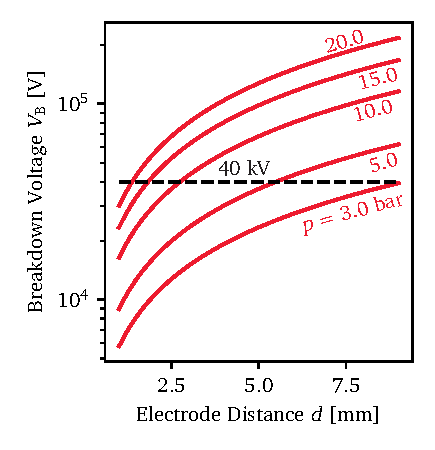
\includegraphics[width=\textwidth]{assets/3 design/pressurePaschen_final}
                    \caption{Required voltage to arc across electrodes}
                    \label{fig:paschenPressure}
                \end{subfigure}
                \hfill
                \begin{subfigure}[t]{0.47\textwidth}
                    \centering
                    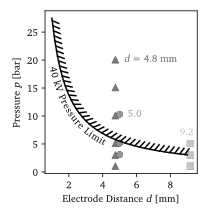
\includegraphics[width=\textwidth]{assets/3 design/sparkTests_final}
                    \caption{Spark tests with varying electrode spacing}
                    \label{fig:sparkTests}
                \end{subfigure}
                \caption{Exploration of spark-gap size in argon with Paschen's law}
                \label{fig:sparking}
            \end{figure}

            This initial model was sufficient to proceed with prototyping spark plugs. Several prototypes were fabricated with varying electrode spacing to determine the maximum electrode gap that could spark across the range of operating pressures. The plugs were then tested to compare their performance to the limit predicted by Paschen's law. The results are shown in \autoref{fig:sparkTests}. One can distinctly see that the spark plugs appear to successfully spark beyond the pressure limit predicted by Paschen. This is thought to be due to the electrode geometry. Indeed, the $\mathsf{A}$ and $\mathsf{B}$ parameters used above were determined for parallel flat plate electrodes, whereas the pointed electrodes are more favorable for arcs by concentrating the electric field near the tips. Furthermore, more sophisticated Particle-In-Cell simulations for spark formation implemented by \textcite{theisComputingPaschenCurve2021} suggest that Paschen's Law overestimates the necessary breakdown voltage for $pd$ values above \qty{10}{Torr.cm}.

            As far as the experiment was concerned, the test showed that a single spark plug with electrodes spaced by 4.8~mm was sufficient to spark throughout the range of operating pressures considered for the experiment. The 4.8~mm gap sparked reliably while still leaving ample space for the laser beam. Initial LSP ignition tests would later show that this design approach is not optimal, as will be discussed in \autoref{sec:ignitiontest}.
        
        \subsection{Thrust stand}
            In order to perform preliminary thrust experiments, the LTTLM would have to be mounted on a custom thrust stand. The design and assembly of this thrust stand was delegated to a team of students collaborating on the project. A\added{ preliminary} set of requirements were given to them, inspired in part by thrust stand designs by \textcite{takkenDevelopmentHightemperatureSolar2021,jansenImprovementValidationTest2016}, which would be verified upon delivery of the thrust stand. \added{As is discussed in detail in \autoref{sec:model_thrust}, the expected thrust at the given laser power levels for an LTP thruster are much lower than stated in requirement TS-2. This requirement was set in part to accommodate for the use of larger nozzles than needed, which would allow for test-section flow velocities on the order of \qty{1}{m.s^{-1}}. As discussed in \autoref{sec:ts_testing}, issues in developing the thrust stand lead to focusing on static LSP tests rather than attempting to take thrust measurements of the LSP-powered thruster.}\comment[id=BZ]{(...) what is the required thrust resolution in the measurements?}\comment[id=ED]{Now discussed in \autoref{sec:model_thrust}}

            \begin{table}[h]
                \renewcommand{\arraystretch}{1.3}
                \centering
                \caption[Top-level design requirements for the thrust stand]{Top-level design requirements for the thrust stand (the ``system'')}
                \label{tab:tsReq}
                \begin{tabular}{l>{\raggedright}p{0.4\textwidth}p{0.4\textwidth}<{\raggedright}}
                    \toprule
                    Identifier  & Requirement   & Rationale \\
                    \midrule
                    TS-1 &  The system shall hold up the thruster such that its thrust axis is horizontal & This ensures the horizontal laser beam can be lined up with the thrust axis \\
                    TS-2 &  The system shall have a maximum measurable thrust rating of at least 10 N, and no greater than 20 N &  The expected operating pressures and nozzles would yield a maximum thrust within that range\\
                    TS-3 &  The system shall provide thrust measurements with a sample rate of at least 1000 S/s & This provides at least 10 thrust readings during a laser pulse \\
                    TS-4 &  The system shall not impede laser focusing into the thruster & The laser must be able to focus into the chamber to sustain LSP \\
                    TS-5 &  The system shall allow known loads to be applied for calibration and preloading & Applying these loads allows correction for friction and backlash in the system \\
                    TS-6 &  The system shall mount to existing optical benchtop & This facilitates integration with the optical hardware \\
                    TS-7 &  The system shall not impede existing measurement equipment & Impeding other instrumentation would limit the type of experiments that can be performed \\
                    \bottomrule
                \end{tabular}
            \end{table}

            

            \begin{figure}[h]
                \centering
                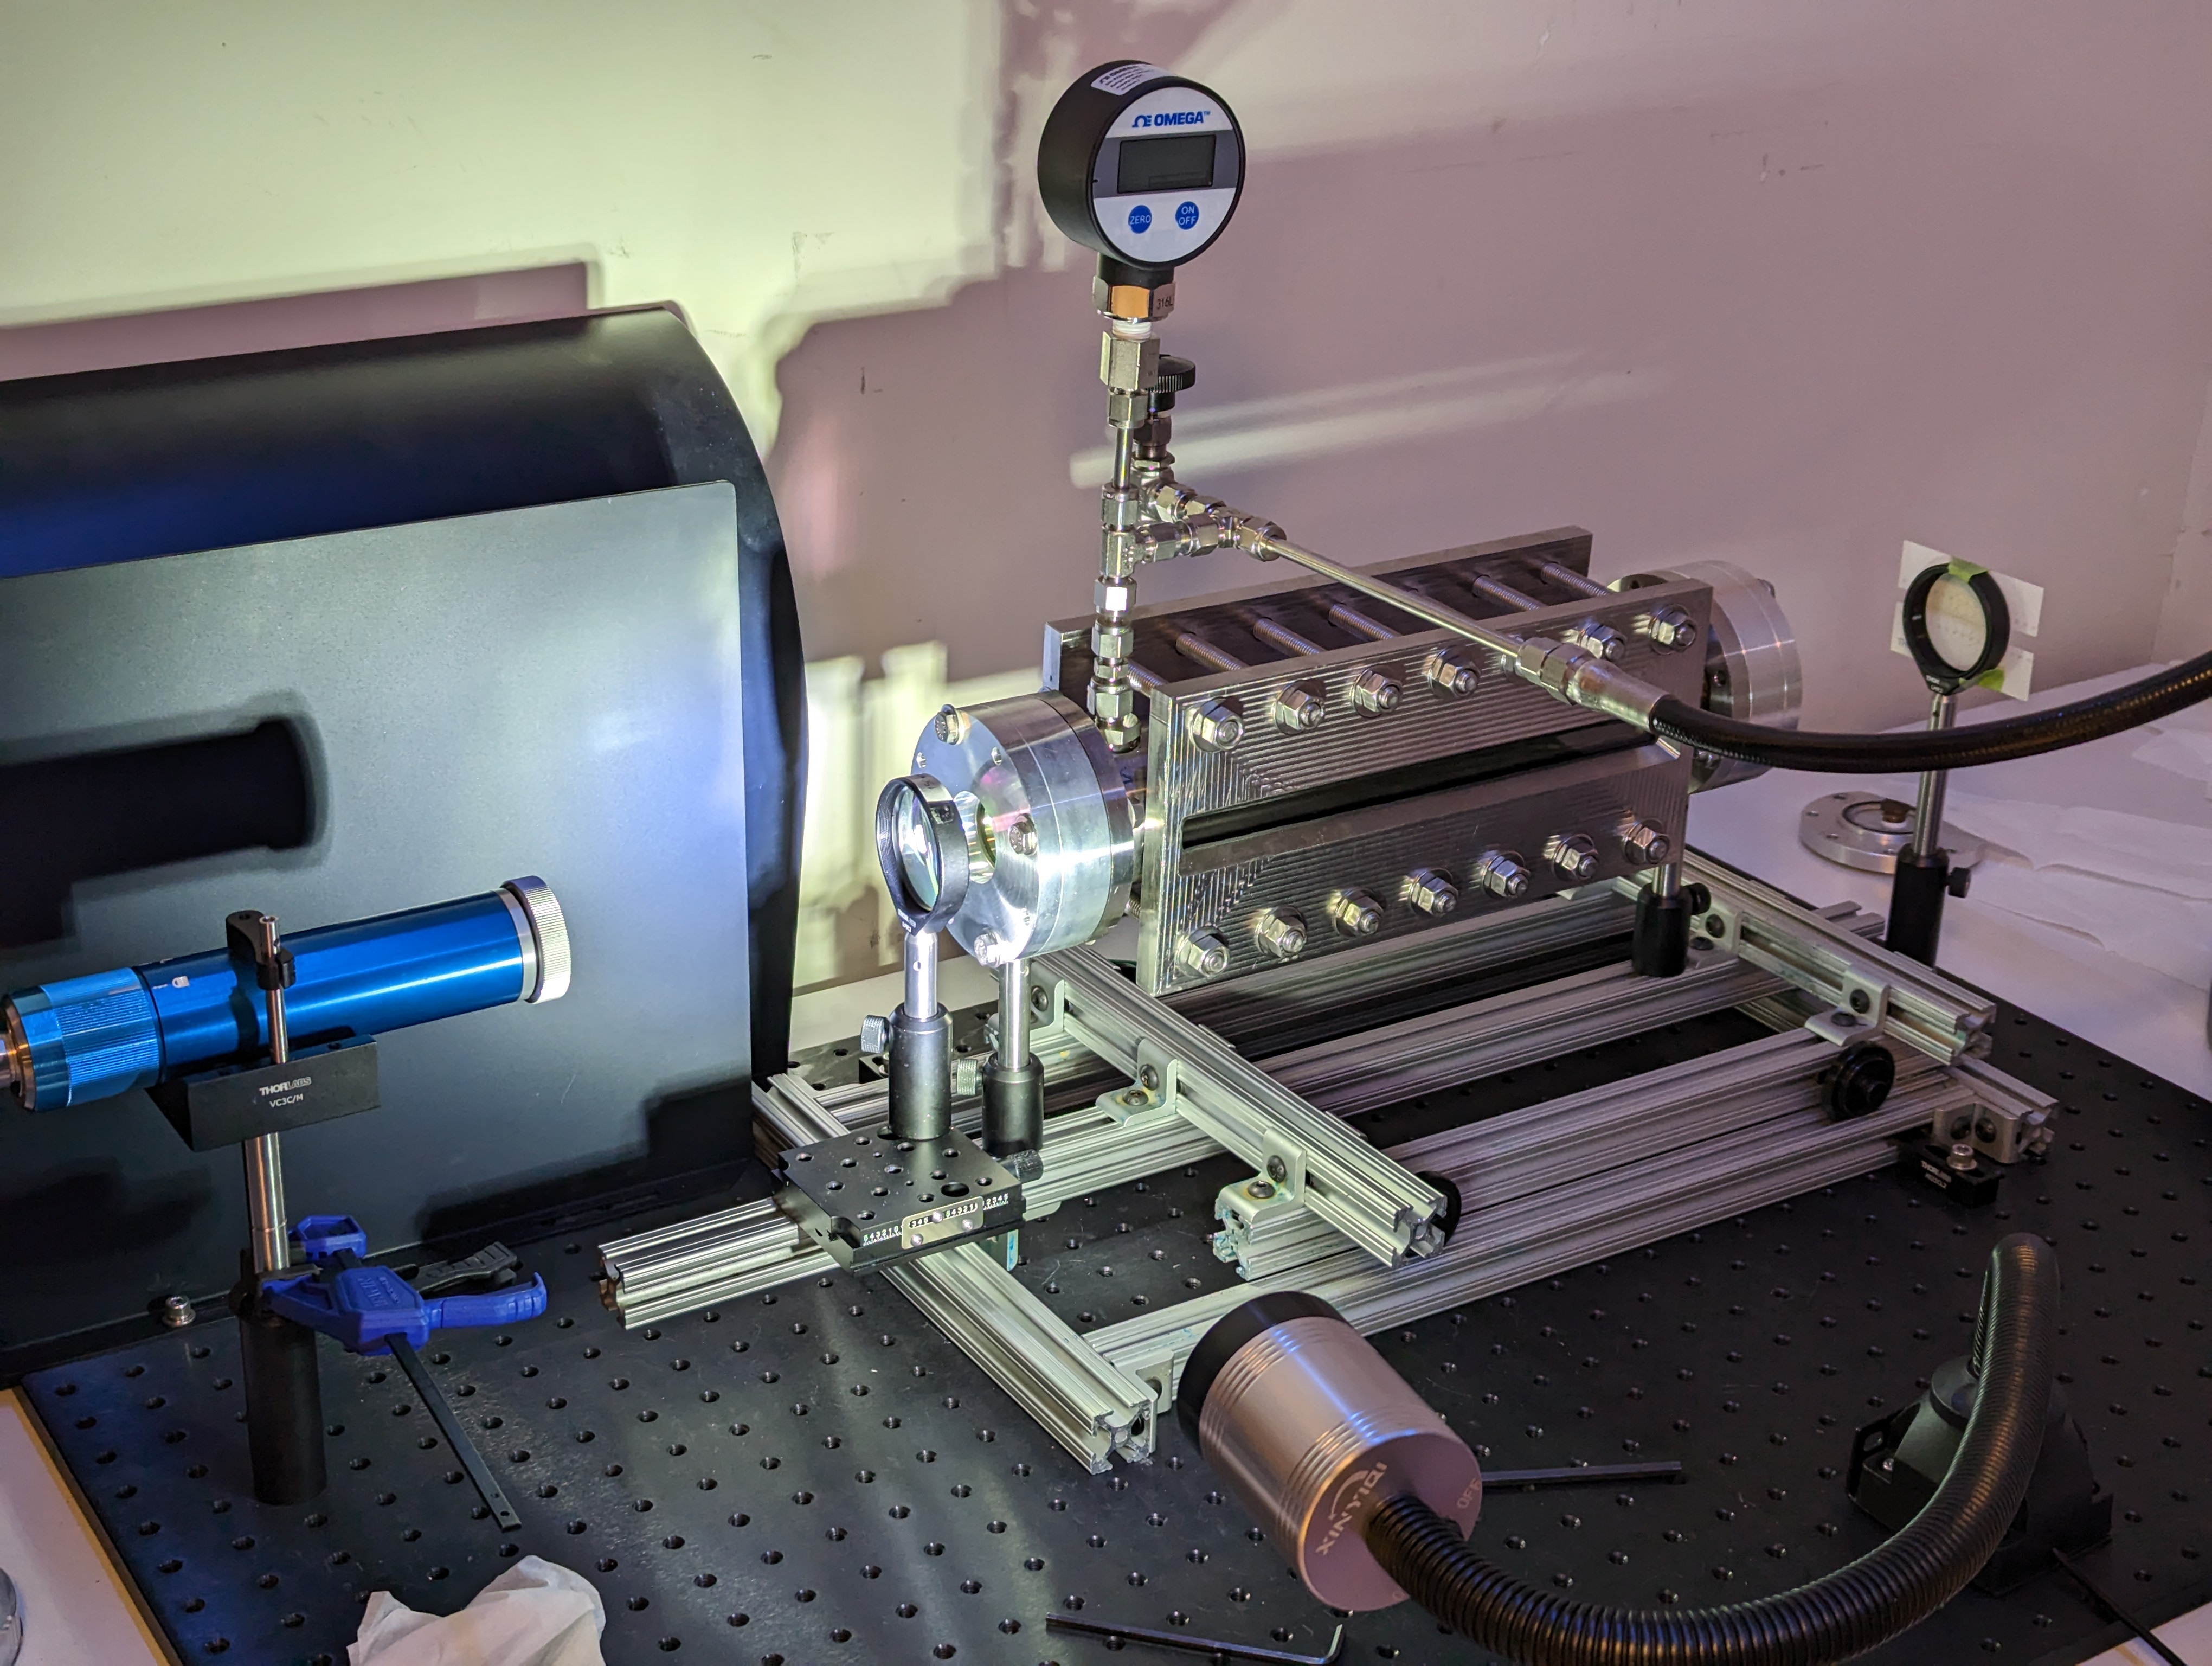
\includegraphics[trim=0 0 0 12in, clip, width=0.67\textwidth]{assets/3 design/thrust_stand.jpg}
                \caption[Test section mounted on the delivered thrust stand]{Test section mounted on the delivered thrust stand. Load cell, DAQ, and preload/calibration system not pictured. \added{Details on the feed system are provided in \autoref{sec:design_integration}.}}
                \label{fig:thrust_stand}
            \end{figure}

            The delivered design (pictured in \autoref{fig:thrust_stand}) consisted of a wheeled cart placed on aluminum extrusion rails, featuring the means to attach several weights to preload the stand. The structural design of the stand satisfied requirements TS-1 and TS-4 through TS-7. Thrust measurement was performed using a Honeywell FSG020WNPB force sensor, whose signal was processed by a DATAQ Instruments DI-2108 data acquisition system. The force sensor's maximum load rating of \qty{20}{N} and the DAQ's \num{50}-\unit{kHz} maximum rate frequency meant that requirements TS-2 and TS-3 were also satisfied. Optical hardware could be mounted onto the cart itself, which facilitated laser alignment with the test section.

    \section{Integration and test}
        As part of the design process and the progressive integration of all the experimental apparatus, a series of tests were performed on various components of the experiment. This was done to verify each component performed as expected and to a degree deemed sufficient for the experiment.
        
        \subsection{Pressure testing}
            One of the first concerns regarding the test section acquired from the FDL was whether it could sustain 20~bar of internal pressure and whether it could maintain this pressure with minimal leakage. Before taking possession of the test section, the FDL demonstrated that it could sustain the necessary \qty{20}{bar} of pressure without failing. They also showed the test section had an average leak rate of \qty{0.04}{bar/min} when pressurized with \qty{11}{bar} of  nitrogen, or a 1.8\% pressure drop over 5 minutes. To determine whether these promising results would be applicable to argon, the leak rates $L$ of two different gases in the same system and conditions can be related by \autoref{eq:leakrates} (\textcite{greenhouseHermeticityElectronicPackages2012}):
            \begin{equation}
                \frac{L_\mathrm{Ar}}{L_{\mathrm{N}_2}} = \sqrt{\frac{\mathcal{M}_{\mathrm{N}_2}}{\mathcal{M}_\mathrm{Ar}}}
                \label{eq:leakrates}
            \end{equation}
            Where the leak rate $L$ is expressed as the product of a volume and pressure loss rate, e.g. \unit{Pa.m^3/s}. Evaluating \autoref{eq:leakrates} with the properties of argon and  nitrogen shows that the test section is expected to leak 16.3\% slower when filled with argon. This provided the confidence needed to move forward with repurposing the FDL's cavitation test section into an LSP generator.
            
            An acceptable leak rate was determined based on the expected time needed to complete an experimental trial after pressurizing the test section. This time is needed to perform laser safety procedures (closing laser curtains, turning on a laser warning light, etc.), power on the laser, check that instrumentation is ready, and more. This was estimated to take 5~minutes, and a 1\% loss in test section pressure was deemed acceptable within that time frame.

            \autoref{fig:pressureTest_og} shows the results of pressure testing the test section as received from the FDL, i.e., fitted with polycarbonate/acrylic side windows, and with the ends sealed with blank endcaps. This was necessary to confirm that similar leak rates could be achieved with argon compared to the nitrogen test, and to serve as a comparison basis once new windows would be integrated in the test section. As seen in \autoref{tab:pressureTests_og} a series of tests were performed at varying argon pressures, with attempts made to minimize leaks. Pressure measurements were read off a digital pressure gauge at 1 minute intervals. Only minor adjustments to the test section fittings were needed to bring the leak rate below the acceptable threshold of 1\% over 5 minutes. 

            \begin{figure}[h]
                \centering
                \begin{subfigure}[t]{0.47\textwidth}
                    \centering
                    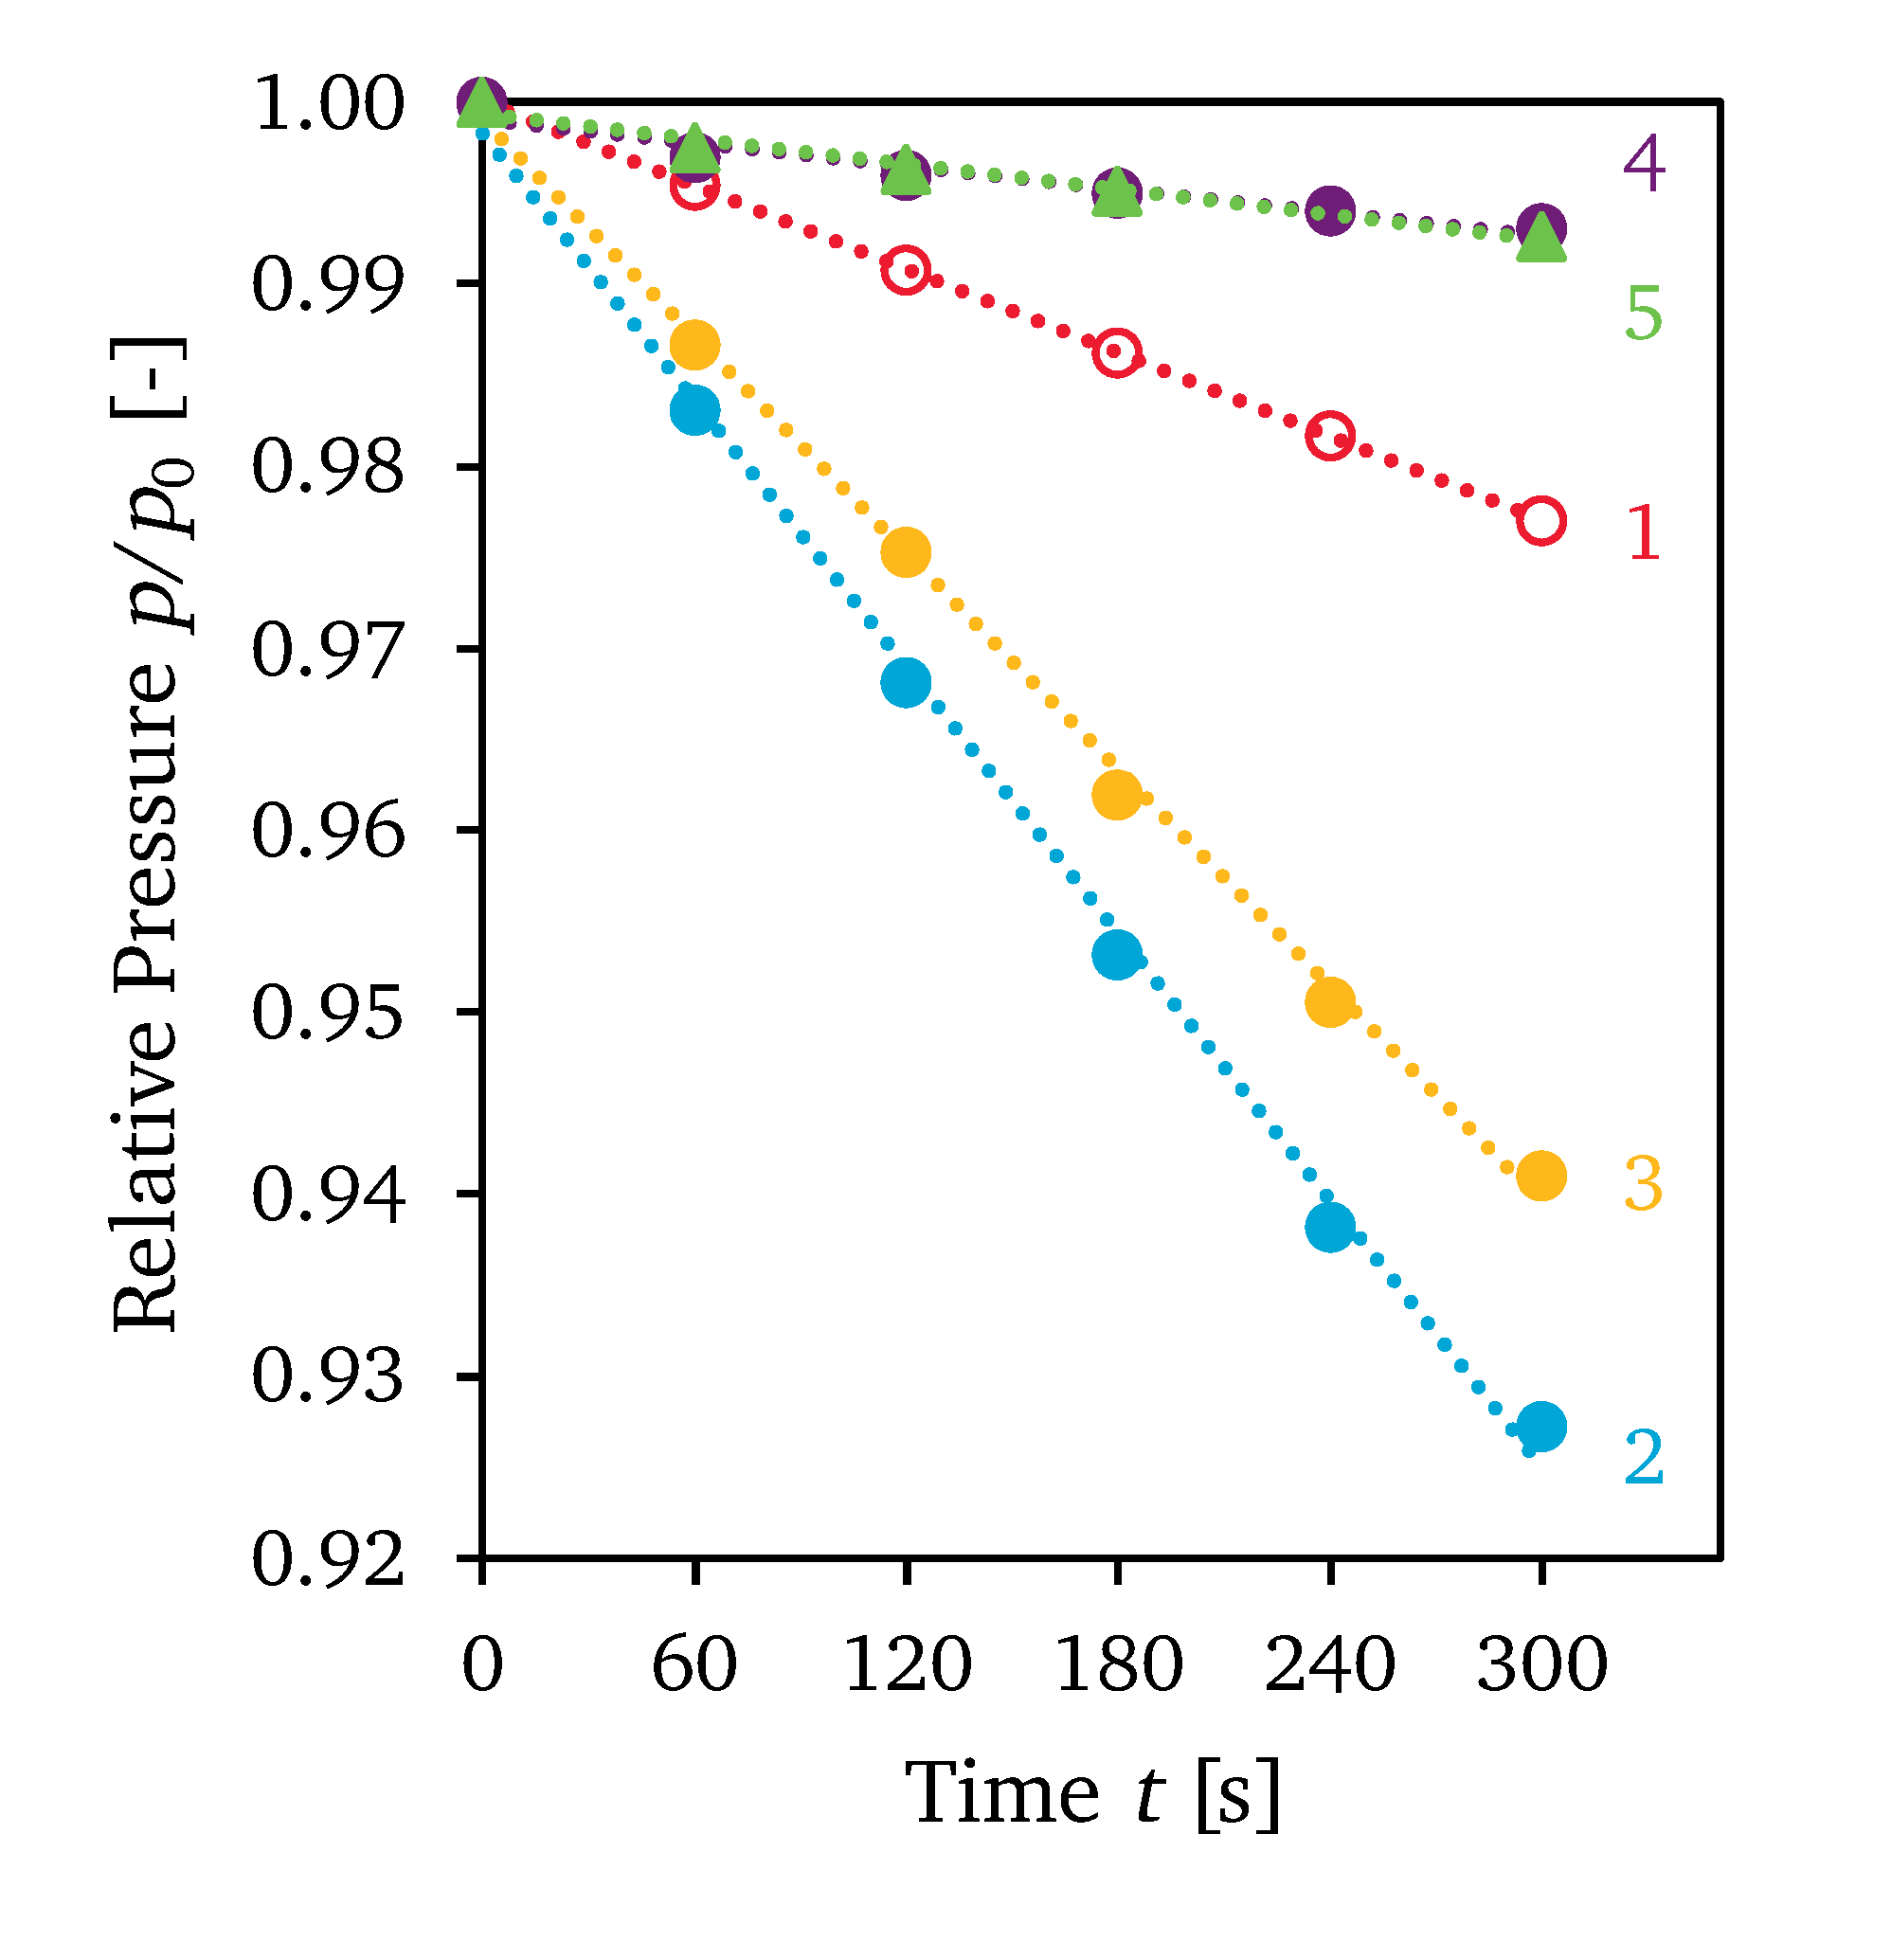
\includegraphics[width=\textwidth]{assets/3 design/pressureTest_original}
                    \caption{As received from the FDL, see \autoref{tab:pressureTests_og} for details}
                    \label{fig:pressureTest_og}
                \end{subfigure}
                \hfill
                \begin{subfigure}[t]{0.47\textwidth}
                    \centering
                    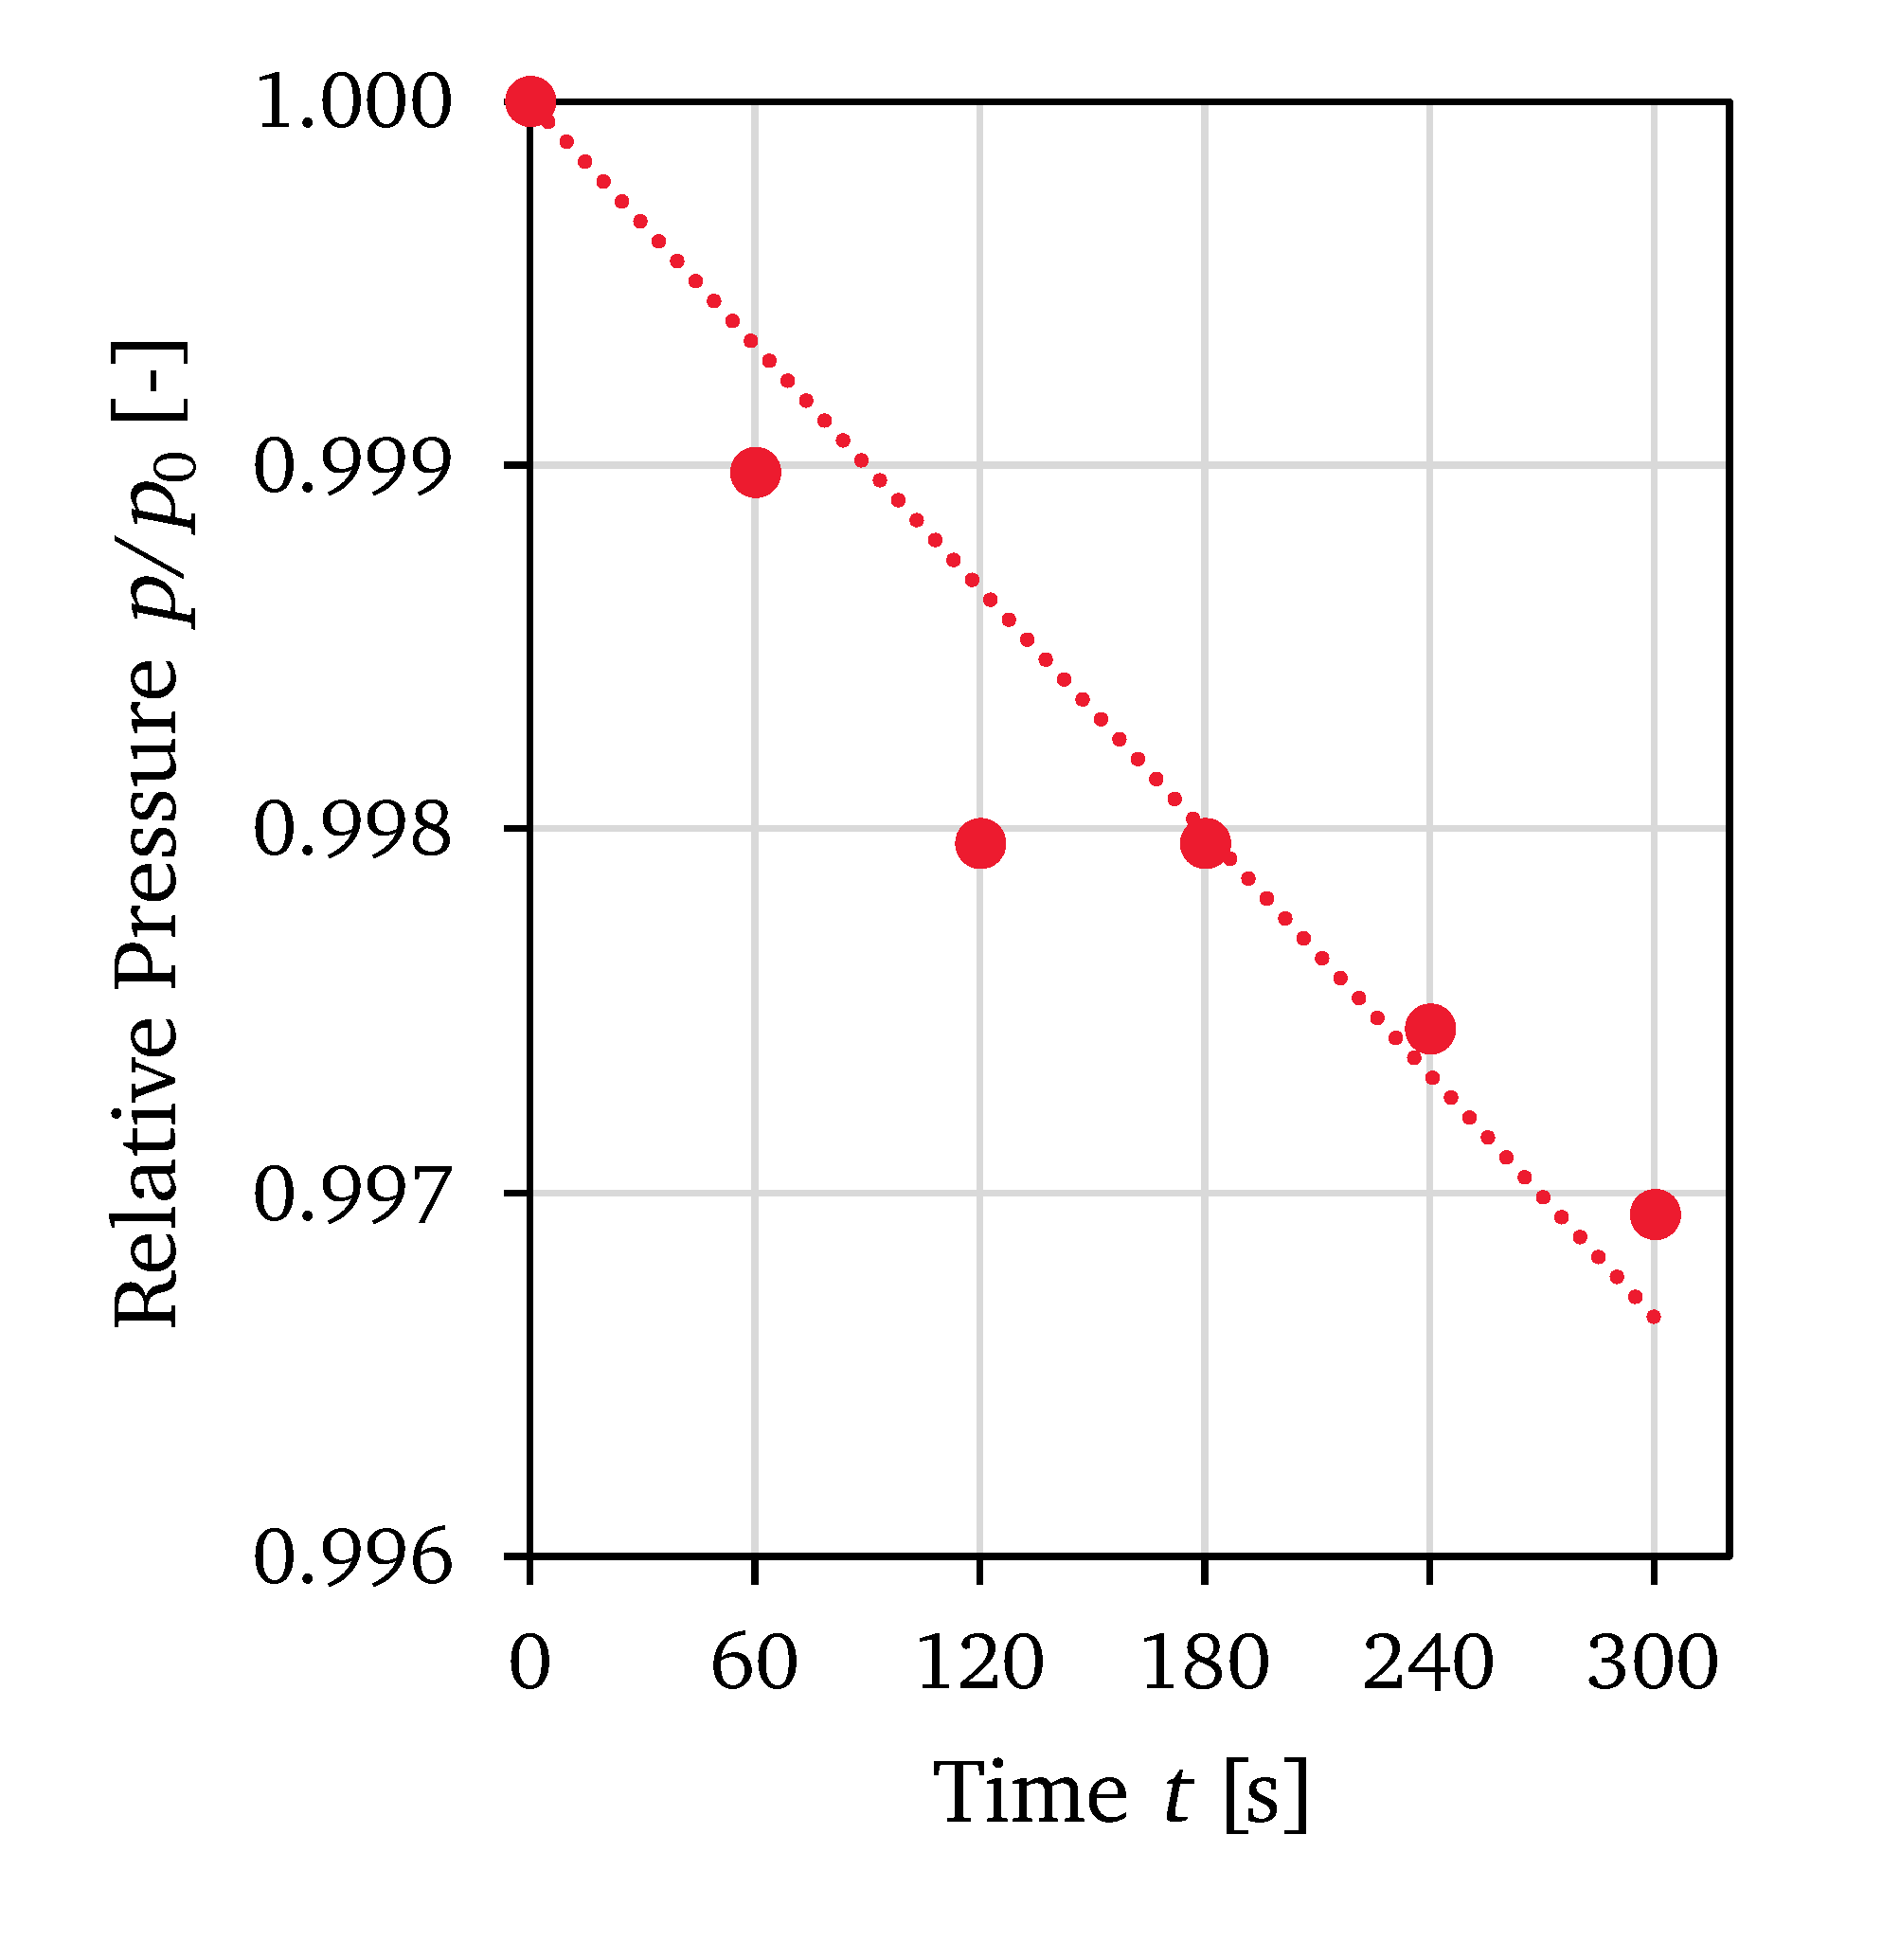
\includegraphics[width=\textwidth]{assets/3 design/pressureTest_newWindows}
                    \caption{With new laser windows and side windows}
                    \label{fig:pressureTest_final}
                \end{subfigure}
                \caption{Pressure leak tests on the test section}
                \label{fig:pressureTest}
            \end{figure}

            \begin{table}[h]
                \centering
                \caption[Pressure leak tests on test section]{Pressure leak tests on test section received from the FDL. The initial pressure is $p_0$, $\overline{\ddi{p}{t}}$ is the average leak rate, and $\Delta p/p_0$ is the relative pressure loss after a specified time.}
                \label{tab:pressureTests_og}
                \begin{tabular}{lrrrl}
                    \toprule
                    Test \#  & $p_0$ [bar]  & $\overline{\ddi{p}{t}}$ [bar/min]   & $\Delta p/p_0$ (5~min) & Comments \\
                    \midrule
                    1   & 3.01  & 0.0138    & 2.3\%    &   \\
                    2   & 6.92  & 0.1007    & 7.3\%    &   \\
                    3   & 7.25  & 0.0855    & 5.9\%    & Tightened plug \#2  \\
                    4   & 6.95  & 0.0097    & 0.7\%    & Replaced vent valve  \\
                    5   & 11.24 & 0.0165    & 0.7\%    &   \\
                    \bottomrule
                \end{tabular}
            \end{table}

            Once the laser windows and UVFS windows were installed, another pressure test was performed to qualify the facility for experimentation. \autoref{fig:pressureTest_final} shows the result of this test, done at an initial pressure of \qty{19.6}{bar}. The test section leaked at an average rate of \qty{0.012}{bar/min}, resulting in a relative pressure loss of 0.3\% after 5 minutes, well within the acceptable rate. The improved leak rate is thought to be due partially to the use of UVFS windows: their smoother surface finish may have provided a better seal, and their susceptibility to fracture meant that careful tightening of the window clamp was required. This was performed with a torque wrench, tightening each bolt of the clamp to \qty{5}{N.m}, following a sequence used for bolting automotive engine cylinder heads. In addition to preventing window fracture, this evenly distributed the clamping load, minimizing the chances of a leak path forming between the window and the gasket.

        \subsection{Laser power tests}
            Laser power and optical power loss tests were necessary to understand the limitations of the laser system and determine the losses induced by the optics in the experiment.

            The YLR-300/3000 laser provides control over the laser power as a setpoint percentage. Early laser tests showed that there was a minimum threshold setpoint under which the laser would not function. Such a phenomenon is implied by the calibration report but is not explicitly documented. As the primary method to control power is through this setpoint percentage system, calibration was required to determine the true useful CW and pulsed power range. To do so, the laser was set up to point directly at the Gentec power meter and turned on over a range of power setpoints. The incident power on the power meter was then recorded.

            The result of this first test run are shown in \autoref{fig:cw_tests}. The power setpoint threshold was found to be at approximately 27\%. This was the point at which a significant signal was detected on the Gentec power meter. The power stability at that threshold is poor when compared to a higher setpoint, as seen in \autoref{fig:cw_tests_time}, and the output power at that setpoint deviates from the otherwise closely linear relationship between setpoint percentage and output power, seen in \autoref{fig:cw_tests_setpoint}. In addition, the maximum CW power appears to significantly exceed the nominal average power rating of the laser, at \qty{350}{W} instead of \qty{300}{W}. Considering these results, the effective operating range (where the power is stable and in the linear range) of the laser in CW mode was deemed to be between 30 and 100\%. A linear fit of the data (for $n_\mathrm{sp} \geq 30$\%) was made to accurately convert a given setpoint $n_\mathrm{sp}$ to an output power $P$, with the resulting affine function printed on \autoref{fig:cw_tests_setpoint}.

            \begin{figure}[h]
                \centering
                \begin{subfigure}[t]{2.5in}
                    \centering
                    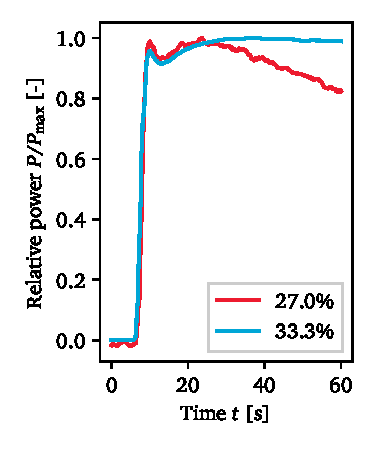
\includegraphics[]{assets/3 design/cw_power_time}
                    \caption{Power stability: the decrease in power seen after the initial peak is due to the power meter's rise time compensation (``anticipation'') feature. This did not affect the calibration results as the steady state measurement was used.}
                    \label{fig:cw_tests_time}
                \end{subfigure}
                \hfill
                \begin{subfigure}[t]{3.3in}
                    \centering
                    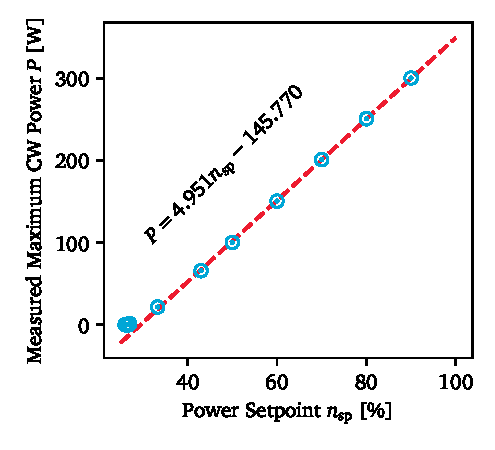
\includegraphics[]{assets/3 design/cw_power_setpoint}
                    \caption{Setpoint percentage to power relation. Blue markers represent experimental tests, the dashed line is a linear fit for the data, excluding points below 30\% of setpoint power.}
                    \label{fig:cw_tests_setpoint}
                \end{subfigure}
                \caption{CW laser output power test results}
                \label{fig:cw_tests}
            \end{figure}

            In the pulsed power regime, similar tests were performed, but found a practically linear relationship. Furthermore, pulsed mode could be controlled with IPG's PulseShaper software, which used calibration settings saved on the laser itself to accurately determine the pulse power/energy. The maximum pulse energy (100\% for \qty{10}{ms}) was \qty{30.8}{J}.

            \subsubsection*{Optical power losses}
                As mentioned in \autoref{sec:design_lwm}, power losses through the focusing optics were expected and tolerated as long as they could be measured and accounted for. The power losses in the system can be characterized by \autoref{eq:powerLosses}:
                \begin{equation}
                    P_\mathrm{m} = P(1-\ell_\mathrm{l})(1-\ell_\mathrm{w})(1-\alpha_\mathrm{LSP})(1-\ell_\mathrm{other})(1-\ell_\mathrm{w})
                    \label{eq:powerLosses}
                \end{equation}
                Where $P$ is the laser power exiting the collimator, $\ell_\mathrm{l}$ is the loss due to the lens, $\ell_\mathrm{w}$ is the loss due to a laser window, $\ell_\mathrm{other}$ are losses due to parts of the test section interior blocking the beam, and $P_\mathrm{m}$ is the measured power at the power meter. The power absorbed by the LSP is also included as $\alpha_\mathrm{LSP}$, and must be determined during experiment. These losses are illustrated in \autoref{fig:sankeyOptics}. If $(1-\ell_\mathrm{l})(1-\ell_\mathrm{w})$ and $(1-\ell_\mathrm{other})(1-\ell_\mathrm{w})$ can be determined separately (although with no need to determine the individual losses due to each component), then they can be accounted for to calculate an accurate value for $\alpha_\mathrm{LSP}$.

                \begin{figure}[h]
                    \centering
                    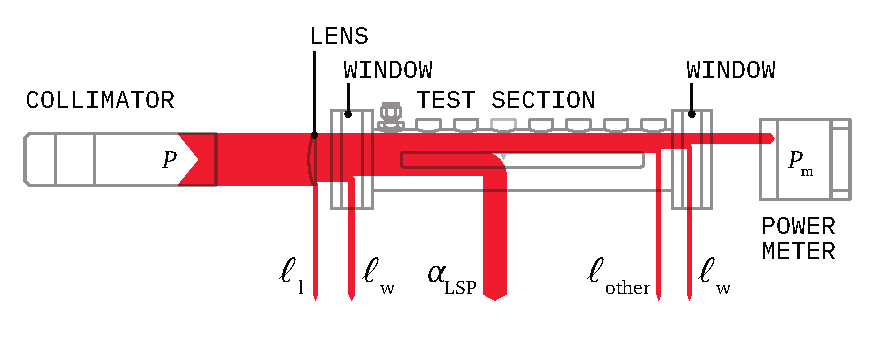
\includegraphics[]{assets/3 design/sankeyOptics}
                    \caption{Qualitative diagram of laser power losses throughout the test section.}
                    \label{fig:sankeyOptics}
                \end{figure}

                To determine these losses, the laser was programmed to output \qty{100}{W} of CW power. Incident power was measured by the Gentec power meter with no optics. Then, the focusing lens and one laser window were placed in the beam path between the laser collimator and the Gentec power meter. The incident power in both cases was measured for 30~s once the power meter's signal reached steady-state (after 60~s). This allows the measurement of $(1-\ell_\mathrm{l})(1-\ell_\mathrm{w})$. A similar procedure was followed to determine $(1-\ell_\mathrm{l})(1-\ell_\mathrm{w})(1-\ell_\mathrm{other})(1-\ell_\mathrm{w})$, by placing the focus lens and the entire test section in the laser beam path. The results of both tests are summarized in \autoref{tab:opticalLoss}.

                \begin{table}[h]
                    \centering
                    \caption{Optical power loss test summary}
                    \label{tab:opticalLoss}
                    \begin{tabular}{lrrrr}
                        \toprule
                        Test        & $P$ [W]   & $P_\mathrm{m}$ [W]    & $P-P_\mathrm{m}$ [W]  & $1-P_\mathrm{m}/P$ [-] \\
                        \midrule
                        Front optics    & 100.19    & 99.60 & 0.587  & 0.586\% \\
                        Full test section    & 100.92    & 95.32 & 5.602  & 5.551\% \\
                        \bottomrule
                    \end{tabular}
                \end{table}

                These results can be used to compute the loss terms as follows:

                \begin{gather*}
                    (1-\ell_\mathrm{l})(1-\ell_\mathrm{w}) = \frac{P_\mathrm{m}}{P} = \frac{99.60}{100.19} = 0.9941 \\
                    (1-\ell_\mathrm{other})(1-\ell_\mathrm{w}) = \frac{P_\mathrm{m}}{P}\frac{1}{(1-\ell_\mathrm{l})(1-\ell_\mathrm{w})} = \frac{95.32}{100.92}\frac{1}{0.9941} = 0.9501
                \end{gather*}
                
                The much greater losses at the exit of the test sections are likely due to the laser beam being reflected or otherwise blocked by parts of the test section itself. This is an issue at the exit rather than at the laser inlet, as the diverging beam makes it more difficult to entirely avoid reflections. However, as these losses are quantified, they can be compensated for during experiments.

        \subsection{Thrust stand testing} \label{sec:ts_testing}
                Although the delivered thrust stand appeared to match the desired requirements, a series of tests were still necessary to develop a calibration procedure and ensure it provided an accurate thrust measurement. It soon became apparent that the friction caused by the test section's weight would pose a challenge.
                
                The static friction in the system provided much of the reaction force against the thrust, meaning reading the system's thrust directly off of the load cell was not possible. Instead, a calibration procedure was performed using known masses pulling on the apparatus. Masses were added to progressively increase the applied load, then removed in the same manner, to provide a calibrated voltage-to-thrust conversion factor in both directions.
                
                Significant hysteresis was also observed in the system: the measured thrust would not return to 0 at the end of a test, remaining instead close to the final ``real'' thrust reading despite the lack of flow. There was therefore low confidence in the accuracy of any thrust profile that was not monotonically increasing. To mitigate this issue, a system of ropes and cables, illustrated in \autoref{fig:thruster_cables}, was set up to relieve some of the weight of the test section on the thrust stand. Although this appeared to resolve hysteresis, this introduced other issues. The load cell's signal was found to be much noisier, and the readings from the system did not seem consistent with the applied loads, whether from known masses or the thruster itself. It is thought that relieving the test section's weight from the thrust stand made it more susceptible to loads and moments imparted by the feed system tubing and misaligned thrust axis and load cell.

                \begin{figure}[h]
                    \centering
                    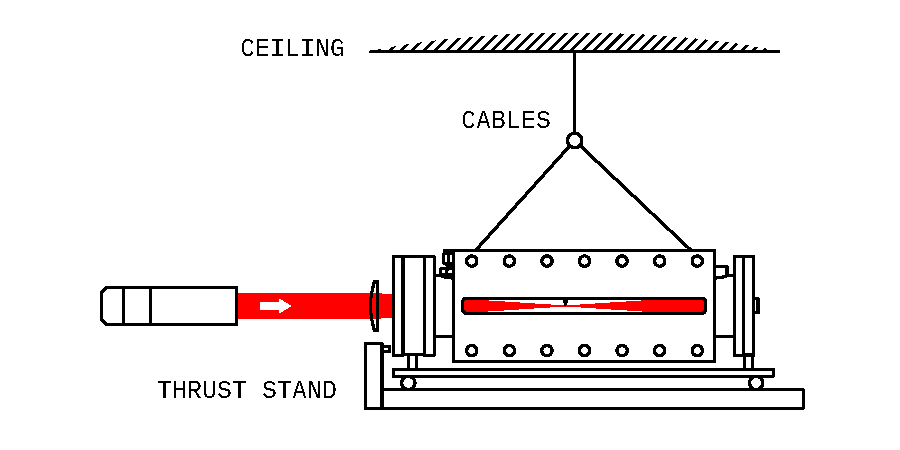
\includegraphics[width=0.9\textwidth]{assets/3 design/thruster_cables}
                    \caption{Diagram of cable system used to relieve thruster weight from the thrust stand}
                    \label{fig:thruster_cables}
                \end{figure}

                In addition to these issues, the problems encountered in other areas of the project including ignition and diagnostics for static LSP, the realization that the deposited heat would likely result in a change in thrust too small to be measured, and the planned design of a dedicated thruster testing model in the future meant that work on the thrust stand was suspended in order to focus efforts on other parts of the project.

        \subsection{System integration} \label{sec:design_integration}
                Once the necessary parts were manufactured, installed, and tested, the experimental apparatus could be integrated together. As the laser pulse duration was short, precise timing and triggering was needed to ensure the necessary conditions for LSP formation, and integration work focused on connecting instrumentation, ignition systems, and the laser such that an entire experimental trial would automatically run with a single trigger. Laser tests and spark tests showed that the laser pulse would begin \qty{2}{ms} after receiving an EMISSION START signal, while the spark would occur at the end of a gate signal which could be controlled to be between \qtyrange{3}{9}{ms}. The experiment was then planned to occur as summarized in \autoref{tab:expTimeline}. This information can also be found in a graphical form in \autoref{fig:timings}, with indications on which triggering signals are active and what they trigger. \added{For flowing tests, a solenoid valve was used to control gas flow---argon was allowed to flow for at least \qty{5}{s} to ensure the test-section pressure stabilized before actually initiating the LSP experiment.}

                \begin{table}[h]
                    % \renewcommand{\arraystretch}{1.3}
                    \centering
                    \caption{Timeline of one experimental run}
                    \label{tab:expTimeline}
                    \begin{tabularx}{\textwidth}{rX}
                        \toprule
                        Time [ms]   & Event \\
                        \midrule
                        0.0         & Experiment is triggered manually. High-speed camera begins recording. Spark-igniter gate signal is opened to charge it. \\
                        6.0         & EMISSION START signal is sent to laser. Oscilloscope begins recording pressure transducer signal. \\
                        8.0         & Laser pulse begins.    \\
                        9.0         & Spark-igniter gate signal closes, spark begins. LSP should begin forming. \\
                        10.0        & Spark should have ended. LSP continues growing.   \\
                        11.0        & Spectrometer begins capturing radiation.  \\
                        15.0        & Spectrometer stops capturing radiation.   \\
                        18.0        & Laser pulse ends, LSP dissipates. \\
                        \bottomrule
                    \end{tabularx}
                \end{table}
                
                \begin{figure}[h]
                    \centering
                    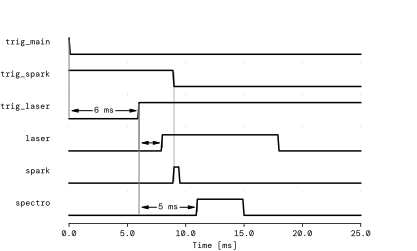
\includegraphics[]{assets/3 design/timings}
                    \caption[Signal timing diagram of an experimental run]{Signal timing diagram of an experimental run. Triggering signals are prefixed with \texttt{trig\_}, all lines indicate whether a component is active (high) or inactive (low). Consult \autoref{tab:expTimeline} for additional details.}
                    \label{fig:timings}
                \end{figure}
                
                % \begin{wrapfigure}{R}{151pt}
                %     \centering
                %     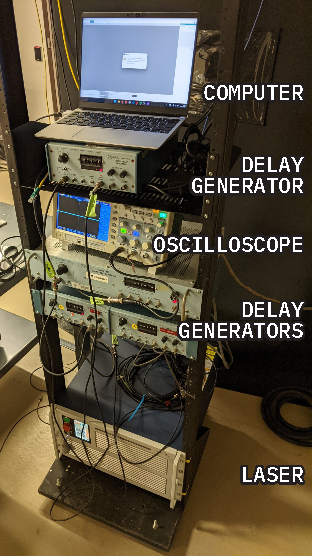
\includegraphics{assets/3 design/setupPhoto_control}
                %     \caption{Experiment control station}
                %     \label{fig:setupPhoto_controls}
                % \end{wrapfigure}

                \paragraph{Experiment control} A series of digital delay generators, seen in \autoref{fig:setupPhoto}, was used to achieve the timings listed shown in \autoref{tab:expTimeline}. These devices use coaxial cables terminated with BNC connectors as inputs/outputs and provide easy adjustment of timings down to sub-\unit{\us} precision, making them ideal to tweak the triggering sequence as the experiment was modified.

                The laser, triggering systems, computer for data acquisition and camera control, and an oscilloscope were mounted on a 19-inch rack, allowing a single operator to run an experiment from the same location. This capability was critical, as the experiment area was contained by laser curtains to protect lab personnel. The oscilloscope was a useful tool to troubleshoot communication between delay generators and other devices, and to monitor the state of the laser at all times.

                \paragraph{Optics} Control over the laser focus was critical to reliably ignite LSP, avoid losing laser power before it reached the power meter, and avoid specular reflections that could damage instrumentation. Several focusing lenses were purchased of varying focal lengths, although all experiments were performed with a \num{200}-\unit{mm} N-BK7 lens. The longer focal length, although not ideal for LSP stability as discussed in \autoref{sec:background_exp}, made it easier to ensure the entire beam would be allowed through the exit window into the power meter, since the beam divergence was smaller. A diagram showing relevant dimensions for optical alignment can be seen in \autoref{chp:app_lwmDrawings}, page \pageref*{chp:app_optics}. The lens was mounted on a set of leadscrew-operated optical stages, allowing precision adjustments to the lens position with 3 degrees of freedom.

                \paragraph{Feed system} Argon gas was provided from a gas cylinder, fitted with a high-pressure regulator, a manual metering valve, and a solenoid valve. Argon was delivered to the test section through 1/4-in tubing. A second manual metering valve was fitted on the tubing to allow venting of the test section. An Omega digital pressure gauge provided a\added{n absolute} static pressure reading of the test section\added{ and was used as the definite measure of test-section pressure when operating the regulator. Mass-flow rates were to be controlled by the choked orifices, as mass-flow meters able to precisely determine flow rates at a high sample rate were not available. This would leave a significant uncertainty on calculated flow rates, but was deemed sufficient at the current stage of the project.}

                \begin{figure}[h]
                    \centering
                    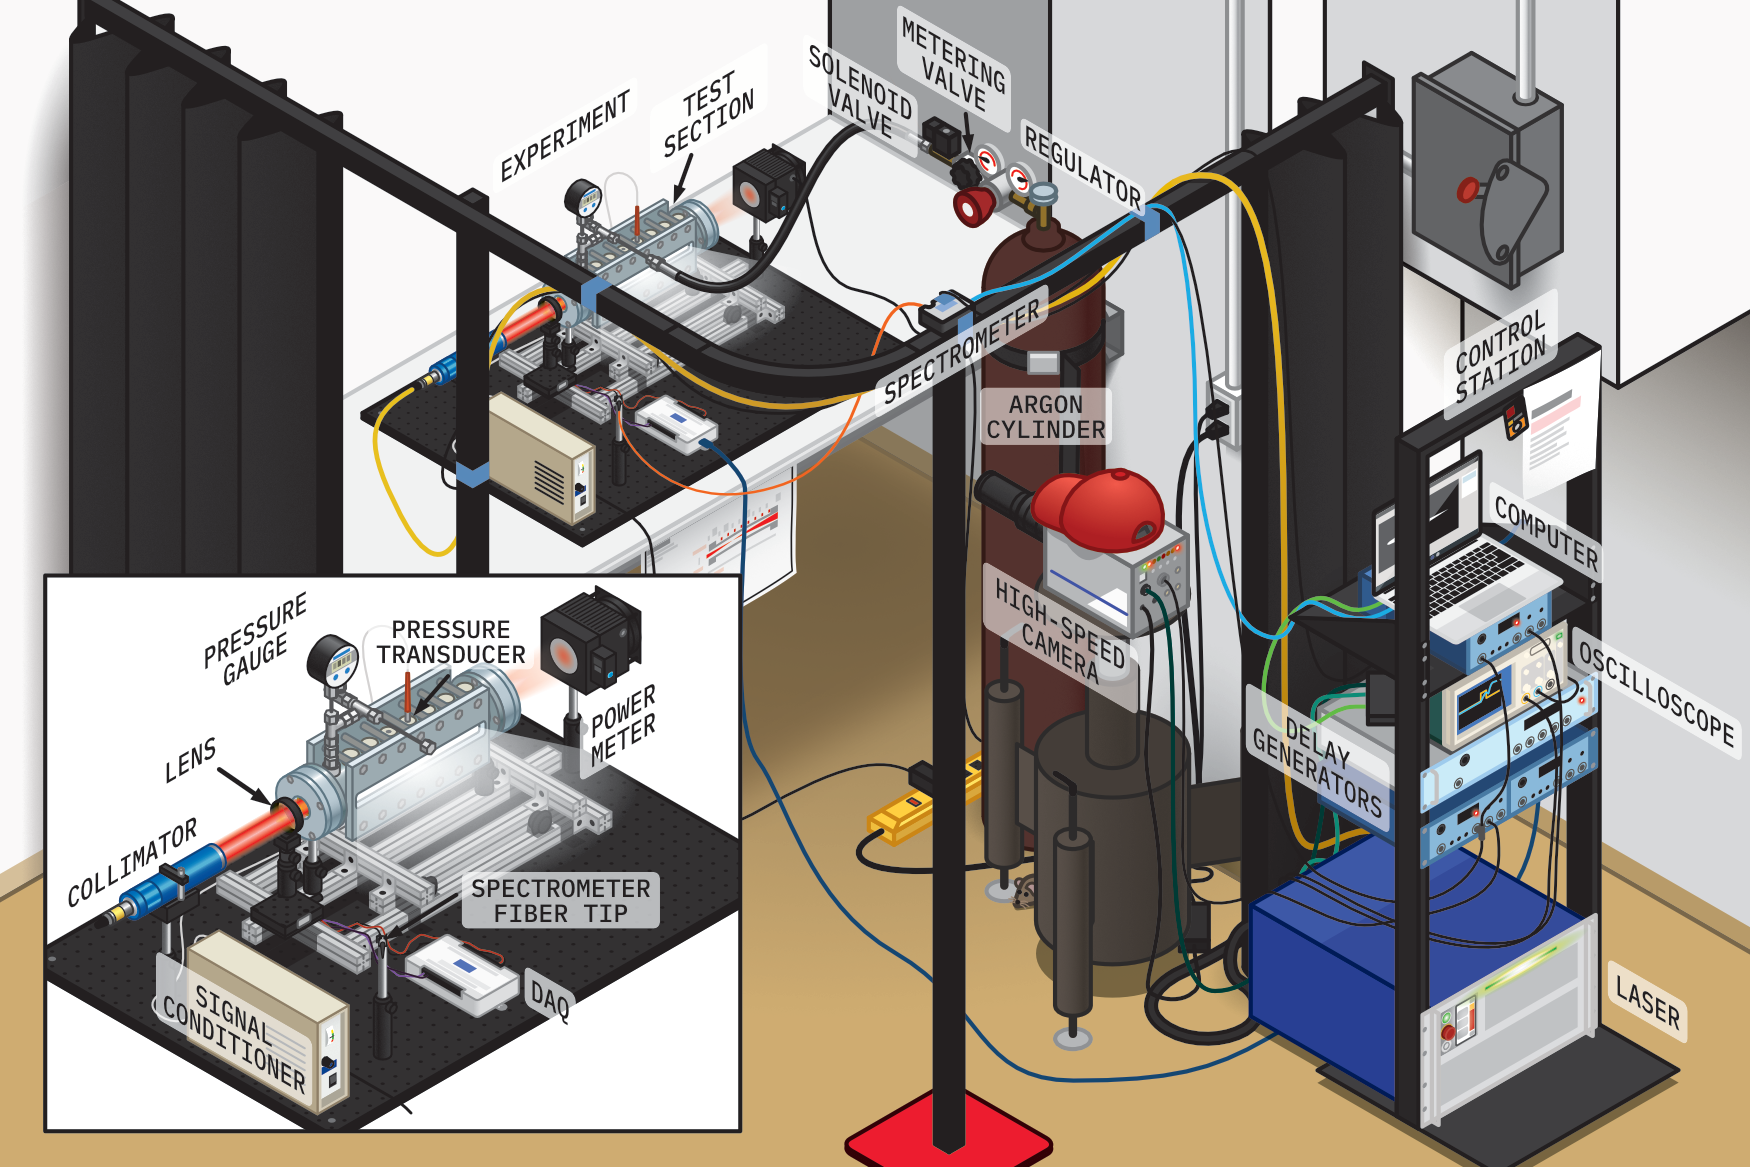
\includegraphics[width=\textwidth]{assets/3 design/setup_isometric.png}
                    \caption[Overview of the experimental setup]{Overview of the experimental setup. Spark igniter is not pictured.}
                    \label{fig:setupPhoto}
                \end{figure}

                % \begin{landscape}
                %     \begin{figure}[h]
                %         \centering
                %         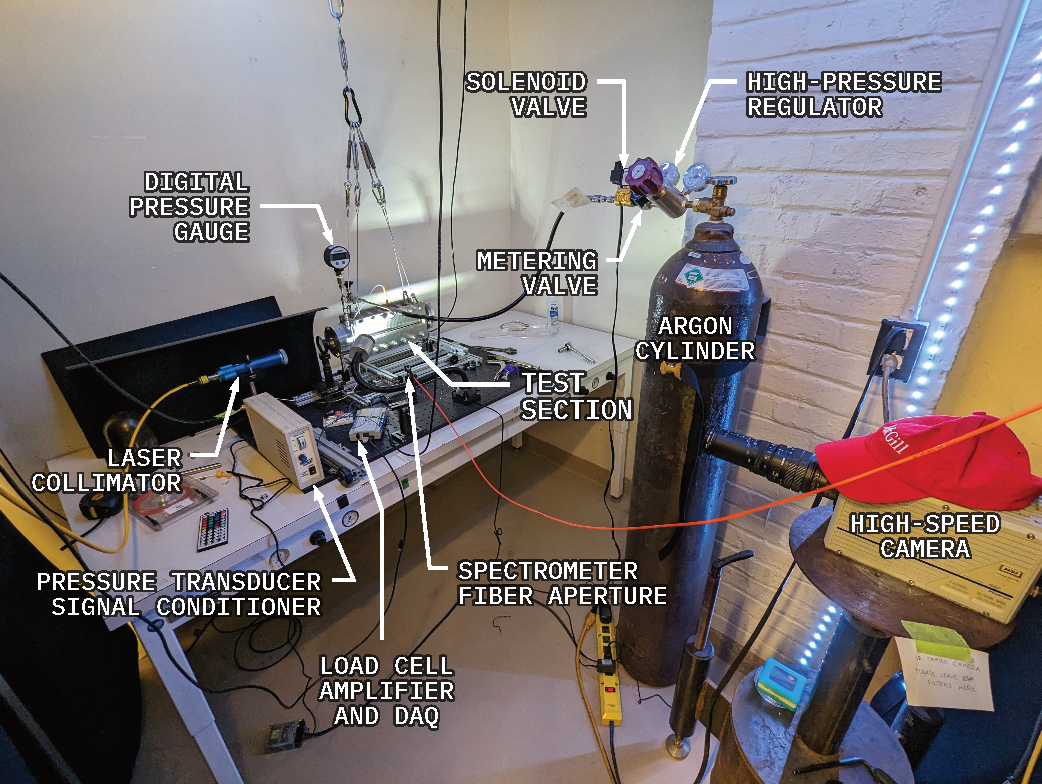
\includegraphics[]{assets/3 design/setupPhoto}
                %         \caption[Experimental setup photograph for flowing tests]{Experimental setup photograph for flowing tests. spark-igniter is not present as this used wire ignition.}
                %         \label{fig:setupPhoto}
                %     \end{figure}
                % \end{landscape}
                % \begin{landscape}
                %     \begin{figure}[h]
                %         \centering
                %         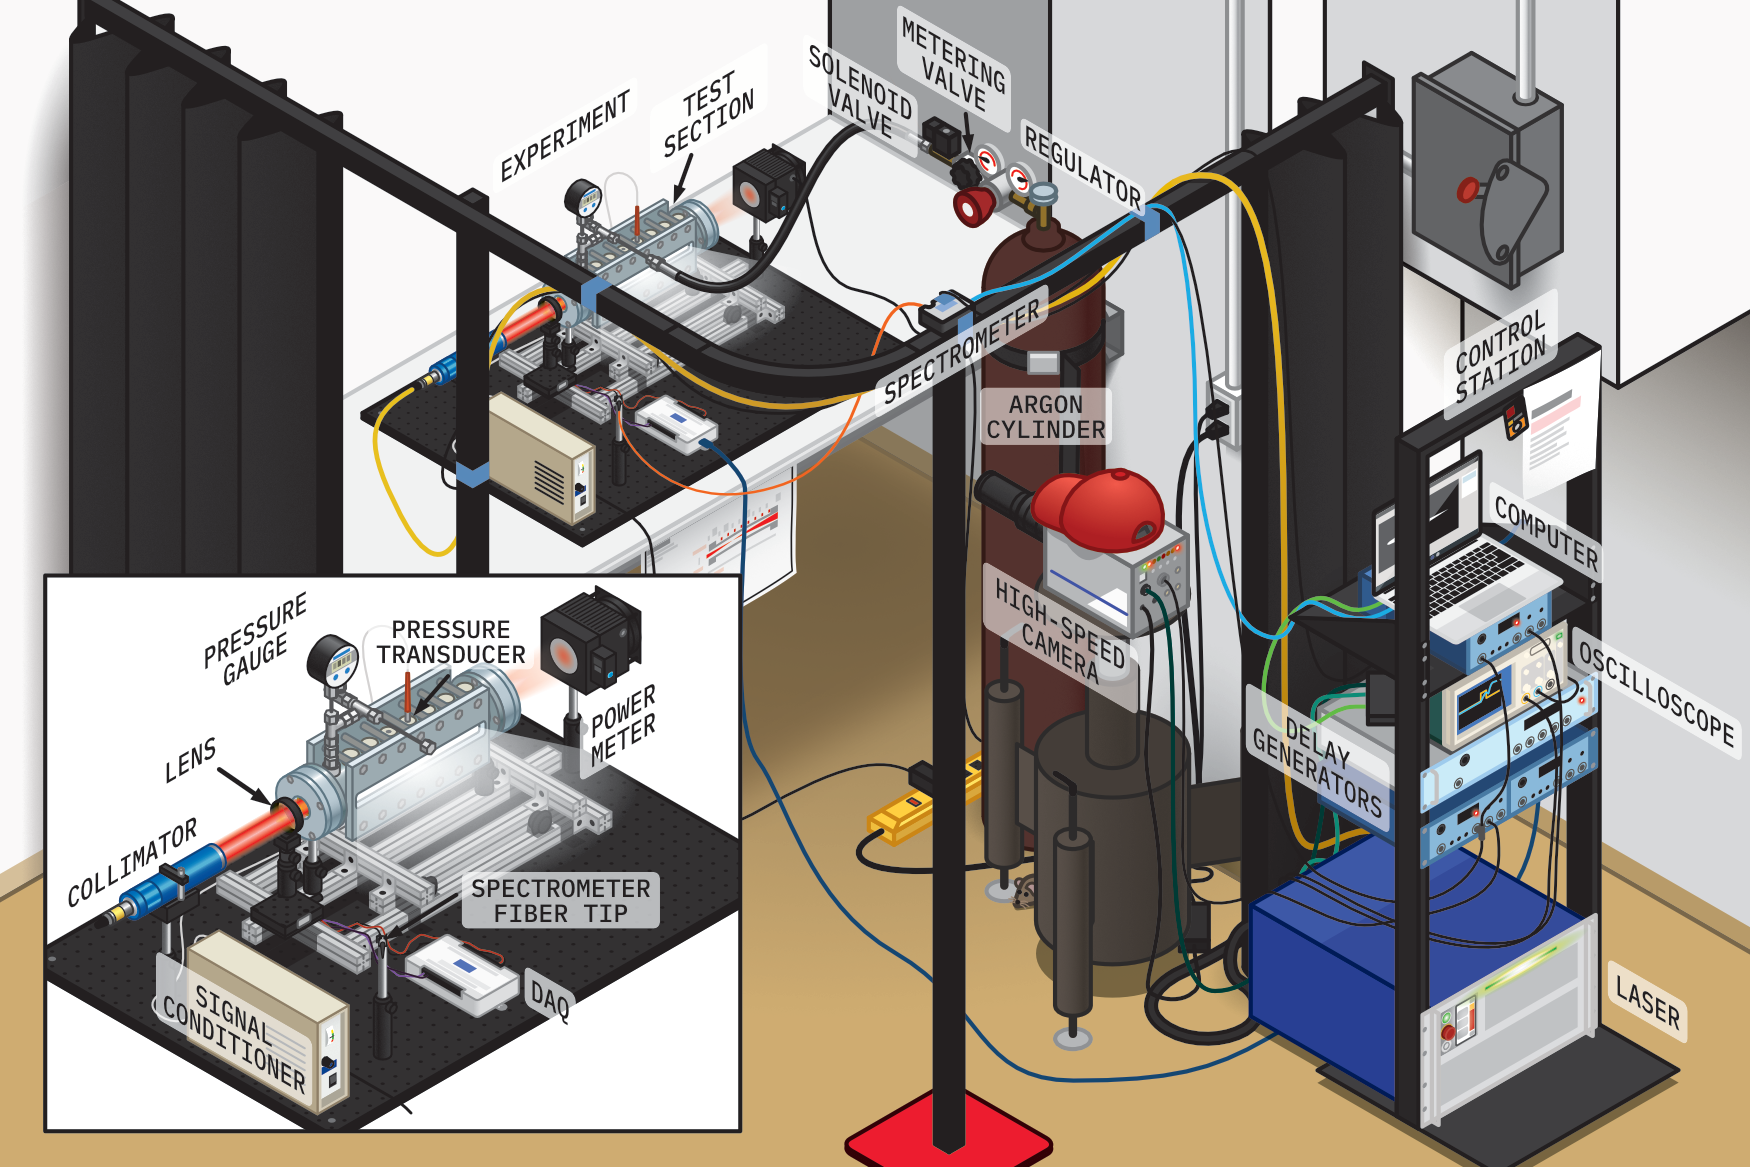
\includegraphics[]{assets/3 design/setup_isometric.png}
                %         \caption[Overview of the experimental setup]{Overview of the experimental setup. spark-igniter is not present as this used wire ignition.}
                %         \label{fig:setupPhoto}
                %     \end{figure}
                % \end{landscape}